\documentclass{article}

\usepackage{geometry}
\usepackage{makecell}
\usepackage{array}
\usepackage{multicol}
\usepackage{setspace}
\usepackage{changepage}
\usepackage{amssymb}
\usepackage{hyperref}
\usepackage{cancel}
\usepackage{amsmath}
\usepackage{fancyvrb}
\usepackage{booktabs}
\usepackage[explicit]{titlesec}
\usepackage{nicefrac}
\usepackage{tocloft}
\usepackage{graphicx}
\usepackage{float}
\DefineShortVerb{\Ħ}
\newcolumntype{?}{!{\vrule width 1pt}}
\renewcommand\theadalign{tl}
\renewcommand{\contentsname}{Inhaltsverzeichnis:}
\newcommand{\paragraphlb}[1]{\paragraph{#1}\mbox{}\\}
\newcommand{\tto}{\ensuremath{\to}}
\setstretch{1.30}
\setlength{\parindent}{0pt}

\newcommand{\N}{\mathbb{N}}
\newcommand{\Z}{\mathbb{Z}}
\newcommand{\Q}{\mathbb{Q}}
\newcommand{\R}{\mathbb{R}}
\newcommand{\M}{\mathbb{M}}

\titleformat{\section}
  {\normalfont\Large\bfseries}{\thesection}{1em}{\hyperlink{sec-\thesection}{#1}
\addtocontents{toc}{\protect\hypertarget{sec-\thesection}{}}}
\titleformat{name=\section,numberless}
  {\normalfont\Large\bfseries}{}{0pt}{#1}

\titleformat{\subsection}
  {\normalfont\large\bfseries}{\thesubsection}{1em}{\hyperlink{subsec-\thesubsection}{#1}
\addtocontents{toc}{\protect\hypertarget{subsec-\thesubsection}{}}}
\titleformat{name=\subsection,numberless}
  {\normalfont\large\bfseries}{\thesubsection}{0pt}{#1}

\hypersetup{
    colorlinks,
    citecolor=black,
    filecolor=black,
    linkcolor=black,
    urlcolor=black
}

\geometry{top=12mm, left=1cm, right=2cm}
\title{\vspace{-1cm}Mathematik für Informatik 1}
\author{Andreas Hofer}

\begin{document}
	\maketitle
	\tableofcontents
	\newpage
	\section{Logik}
	\subsection{Aussagen}
	\subsubsection{Aussageformen}
	Eine Aussage ist ein Satz von dem man eindeutig entscheiden kann wie war er ist. \\
	Eine Aussageform ist hingegen ein Satz mit mindestens einer Variable, wodurch der Wahrheitsgehalt der Aussage nicht eindeutig ist. Ersetzt man in einer Aussage eine Konstante (Ein Wort) durch eine Variable (x), wird diese zu einer Aussageform oder zu einer Aussagefunktion a(x).
	\begin{itemize}
		\item{Wenn man sich zum Beispiel diese Aussagen ansieht:}
		\begin{itemize}
			\item{Graz ist die Hauptstadt von Österreich $\to$ Falsch}
			\item{Wien ist die Hauptstadt von Österreich $\to$ Wahr}
		\end{itemize}
		\item{Hier kann man Graz und Wien durch \textit{x} ersetzen um dieses in eine Aussagenform zu verwandeln: \textit{x} ist die Hauptstadt von Österreich}
		\item{a(Graz) $\to$ Falsch}
		\item{a(Wien) $\to$ Wahr}
	\end{itemize}
	\subsubsection{Verknüpfung von Aussagen}
	Man kann Aussagen auch mit und / oder verknüpfen.
	\begin{itemize}
		\item{UND Verknüpfung oder Konjunktion ($a \land\  b$) ist nur wahr wenn beide verknüpften Elemente Wahr sind.}
		\item{ODER Verknüpfung oder Disjunktion ($a \lor\  b$) ist Wahr sobald eines der beiden Elemente Wahr ist. Sie ist nur Falsch, wenn beide der Aussagen Falsch sind.}
		\item{ENTWEDER ... ODER (XOR) oder Kontravenz ($a \veebar\  b$) ist genau dann wahr, wenn entweder a oder b wahr sind, aber nicht gleichzeitig. Somit ist sie gleich wie die ODER Verknüpfung, wobei sie nicht wahr ist, wenn beide Wahr sind.}
		\item{VERNEINUNG oder Negation ($\neg  a$) kehrt den Gehalt einer Aussage um. So ist ein Element das Wahr ist, danach Falsch.}
	\end{itemize}
	\subsubsection{Wahrheitstabellen}
	Man kann diese Aussagen auch anhand einer Tabelle festlegen: \\ \\ 
	\begin{tabular}{| c | c | c | c | c | c | c |}
		\toprule
		a & b & $a \land\ $  b & a$ \lor\ $  b & $a \veebar\  b$ & $\neg a$ & $\neg b$ \\ \midrule
		0 & 0 & \textbf{0} & \textbf{0} & \textbf{0} & \textbf{1} & \textbf{1} \\ \hline
		0 & 1 & \textbf{0} & \textbf{1} & \textbf{1} & \textbf{1} & \textbf{0} \\ \hline
		1 & 0 & \textbf{0} & \textbf{1} & \textbf{1} & \textbf{0} & \textbf{1} \\ \hline
		1 & 1 & \textbf{1} & \textbf{1} & \textbf{0} & \textbf{0} & \textbf{0} \\
		\bottomrule
	\end{tabular}
	\subsubsection{Beispiel}
	Verneinen Sie folgende Aussageformen:
	\begin{enumerate}
		\item{$a(x): x^2 + 3 > 21 \to \neg a(x):x^2+3 \leq\ 21$}
		\item{$b(x): x^2 + x = 8 \to \neg b(x): x^2+x \neq 8$}
		\item{$\neg c(x): 4x \geq\ 5 \to c(x): 4x < 5$}
	\end{enumerate}

	\subsection{Quantoren}
	\subsubsection{All Quantor}
	Eine All-Aussage setzt voraus, dass gegeben für eine Aussageform a(x), alle \textit{x} aus einer bestimmten Menge wahr sind. \\
	Kurzschreibweise - All Quantor: \\
	$\forall x:a(x)$ \\
	Beispiel:\\
	Aussageform a(x) = x ist die Hauptstadt Österreichs. \\
	Diese Behauptung ist dann wahr, wenn für alle \textit{x} a(x) wahr ist. \\
	Widerlegung: Ein \textit{x} existiert für welches a(x) nicht gilt.
	\subsubsection{Existenz Quantor}
	Eine Existenzaussage ist dann wahr, wenn zumindest eines von einer Menge aus \textit{x} wahr ist. \\
	Kurzschreibweise:
	$\exists x:a(x)$ \\
	Beispiel:\\
	Aussageform a(x) = x ist die Hauptstadt von Österreich \\
	Wahrheitsbeweis: Ein x ist zu finden für welches a(x) wahr ist. \\
	Widerlegung: Für alle \textit{x} in der Menge beweisen, dass a(x) nicht wahr ist.
	\subsubsection{Verneinung}
	Durch die Verneinung werden die Quantoren negiert: \\
	Aus einer All-Aussage wird eine Existenzaussage und aus einer Existenzaussage wird eine All-Aussage. \\

	Beispiel einer All-Aussagennegierung: \\
	$\neg(\forall x:a(x)) = \exists x:\neg(a(x))$ \\
	a(x) = x ist die Hauptstadt Österreichs. \\
	Bei Verneinung der All-Aussage von a(x) wird 'Alle x sind Hauptstädte Österreichs' zu 'Es existiert zumindest eine Hauptstadt Österreichs in x'. \\
	Beispiel einer Existenzaussage: \\
	$\neg (\exists x:a(x)) = \forall x:\neg (a(x))$
	Bei Verneinung der Existenzaussage wird aus 'Es existiert ein \textit{x} in der Menge, welche die Hauptstadt Österreichs ist.' zu 'Es existiert kein \textit{x} welches die Haupstadt Österreichs ist.'
	\subsubsection{Beispiel}
	\begin{enumerate}
		\item{Zu jedem Schloss passt ein Schlüssel $\to$ Es gibt mindestens ein Schloss zu dem kein Schlüssel passt.}
		\item{Es gibt einen Studierenden, der Java nicht kann $\to$ Alle Studierenden können Java.}
		\item{Für alle \textit{x} gilt: \textit{f}(x)$\neq$ 0 $\to$ Es existiert ein x für das gilt: \textit{f}(x) = 0}
		\item{$\forall \textit{x}:10x+4\geq\ 10 \to \exists \textit{x}:10x + 4 \geq\ 10$}
		\item{$\exists \textit{x}: 12 = 2x^2+3x \to \forall \textit{x}:12 \neq\ 2x^2+3x$}
	\end{enumerate}
	\subsubsection{Implikation}
	Bei der Implikation folgt aus einer Aussage eine andere. Wenn a dann b oder a impliziert b.\\
	Kurzschreibweise: \\
	$a \implies b$ \\
	\textbf{Diese Aussage ist nur falsch wenn a wahr und b falsch ist.} \\
	Beispiel: \\
	a(x) = x ist die Hauptstadt von Österreich \\
	b(x) = x ist in Österreich \\
	$a \implies\ b$: Wenn x die Hauptstadt von Österreich ist, muss diese in Österreich liegen. \\
	a = Wien ist die Hauptstadt von Österreich \\
	b = Graz ist die Hauptstadt der Steiermark \\
	$a \implies\ b$ ist Wahr, nicht weil es eine logische Verbindung gibt, sondern weil beide Wahr sind. \\
	a = Wien ist die Hauptstadt Österreichs \\
	b = Graz ist die Hauptstadt Österreichs \\
	$a \implies\ b$ ist Falsch, da a wahr, aber b falsch ist. \\
	Die Logik des genannten Satzes ist in diesem Fall irrelevant. Eine Implikation ist nur dann falsch, wenn a wahr und b falsch ist.
	\paragraphlb{Verneinung}
	Eine Implikation ist auch wahr, wenn beide Aussagen, welche zu einer Wahren Implikation führen, negiert werden. \\
	$a \implies\ b$ - Wahr \\
	$\neg a\implies\ \neg b$ - Wahr
	\subsubsection{Äquivalenz}
	Eine Äquivalenz besteht in nur zwei Fällen. Eine Äquivalenz ausgeschrieben ist \textbf{genau wenn ... dann}. Eine Äquivalenz ist Wahr wenn beide Teile den gleichen Wahrheitswert besitzen. Also ist es wahr wenn a und b Wahr sind, aber auch Wahr wenn a und b Falsch sind. \\
	Kurzform: \\
	$a \iff\ b$

	Wahrheitstabellen: \\
	\begin{tabular}{| c | c | c | c |}
		\toprule
		a & b & $a \implies\ b$ & $a \iff\ b$ \\ \midrule
		0 & 0 & 1 & 1 \\ \hline
		0 & 1 & 0 & 0 \\ \hline
		1 & 0 & 1 & 0 \\ \hline
		1 & 1 & 1 & 1 \\
		\bottomrule
	\end{tabular} \\ \\
	Wahrheitstabelle von $\neg (\neg a \lor\ \neg b)$ \\
	\begin{tabular}{| c | c | c | c | c | c |}
		\toprule
		a & b & $\neg a$ & $\neg b$ & $\neg a \lor\ \neg b$ & $\neg $\\ \midrule
		0 & 0 & 1 & 1 & 1 & 0 \\ \hline
		0 & 1 & 1 & 0 & 1 & 0 \\ \hline
		1 & 0 & 0 & 1 & 1 & 0 \\ \hline
		1 & 1 & 0 & 0 & 0 & 1 \\
		\bottomrule
	\end{tabular} \\ \\
	Diese Tabelle zeigt, dass das De Morgan'sche Gesetz zutrifft. Durch die Negation von $\neg a\lor\neg b$ erhält man $a\land b$.
	\subsubsection{Tautologie}
	Eine Tautologie ist eine allgemeingültige Aussage. Logisch gesehen ist sie somit in jedem Fall wahr. Ein Beispiel wäre 'Wenn es regnet, dann regnet es.' \\
	Mathematisches Beispiel: \\
	$\neg (a \land \neg a)$ Diese Formel ist immer wahr, da a und nicht a nie wahr sind, aber negiert immer wahr ist. \\
	Beispiel: \\
	Ist $ (X \implies\ 1) \implies\ (0 \implies\ Y)$ eine Tautologie? \\
	\begin{tabular}{| c | c | c | c | c |}
		\toprule
		X & Y & $X \implies\ 1$ &$ 0 \implies\ Y$ & $\implies$ \\ \midrule
		0 & 0 & 1 & 1 & 1 \\ \hline
		0 & 1 & 1 & 1 & 1 \\ \hline
		1 & 0 & 1 & 1 & 1 \\ \hline
		1 & 1 & 1 & 1 & 1 \\
		\bottomrule
	\end{tabular}
	\subsubsection{Kontradiktion}
	Eine Kontradiktion ist immer Falsch, da die beiden Aussagen in einem Widerspruch zueinander stehen. \\
	Beispiel: \\
	$a \land\ \neg a$
	Die Erde ist rund und die Erde ist nicht rund. \\

	Ist folgende Formel eine Tautologie, Kontradiktione oder keines von Beiden: \\
	$((a \implies\ b) \land\ (b \implies\ c)) \implies\ (a \implies\ c)$ \\ \\
	\begin{tabular}{| l | l | l | l | l | l | l | l |}
		\toprule
		a & b & c & $a \implies\ b$ & $ b \implies\ c $ & $\lor\ $ & $a \implies\ c$ & $\implies\ $ \\ \midrule
		0 & 0 & 0 & 1 & 1 & 1 & 1 & 1 \\ \hline
		0 & 0 & 1 & 1 & 1 & 1 & 1 & 1 \\ \hline
		0 & 1 & 0 & 1 & 0 & 0 & 1 & 1 \\ \hline
		0 & 1 & 1 & 1 & 1 & 1 & 1 & 1 \\ \hline
		1 & 0 & 0 & 0 & 1 & 0 & 0 & 1 \\ \hline
		1 & 0 & 1 & 0 & 1 & 0 & 1 & 1 \\ \hline
		1 & 1 & 0 & 1 & 0 & 0 & 0 & 1 \\ \hline
		1 & 1 & 1 & 1 & 1 & 1 & 1 & 1 \\ 
		\bottomrule
	\end{tabular}
	Dieser Ausdruck ist somit eine Tautologie.
	\section{Mengenlehre}
	Eine Menge ist eine Zusammenfassung von Objekten, welche gemeinsame Eigenschaften haben. Ein Beispiel sind die Zahlen von 1 bis unendlich. Wichtig ist dabei, dass die Objekte wohl unterscheidbar sind, also darf es keine zwei selben Zahlen innerhalb einer Menge geben. \\
	Das Element \textit{x} wird als wohl unterscheidbares Objekt dargestellt.
	\subsection{Beschreibung von Mengen}
	Mengen werden üblicherweise mit Großbuchstaben bezeichnet: \textit{A, B, M}. Die geschwungenen Klammern \{\} werden auch Mengenklammern genannt und bezeichnen eine Menge. \\
	Die beiden Verfahren zur Beschreibung einer Menge sind: \\
	$M=\{x_1,x_2,x_3\}$ $\to$ Aufzählendes Verfahren \\
	$M=\{x \in A$|x hat bestimme Menge\} \\
	Beispiele sind: \\
	$M=\{0,1,2,3,4,5,6,7\}$ $\to$ Die Menge der Zahlen von 0 bis 7 \\
	$M=\{x\in \Z | -2 > x > 2\}$ Die Menge aller ganzen Zahlen zwischen -2 und 2\\
	$M=\{x\in \Z | -1 \leq x < 7\}$
	\subsubsection{Teil und Nicht Teil}
	Das Symbol $\in$ beschreibt, dass das Objekt ein Element der Menge ist. \\
	Hingegen beschreibt das Symbol $\notin$ dass, das Objekt nicht Teil der Menge ist.
	\subsubsection{Mächtigkeit}
	Die Mächtigkeit einer Menge beschreibt die Anzahl der Elemente einer Menge. \\
	Schreibweise: $|M|$ (Kardinalzahl) \\
	Beispiele: \\
	$M=\{0,1,2,3,4,5\}, |M| = 7$ \\
	$|\N|$ $\to$ "abzählbar unendlich" \\
	$|\R|$ $\to$ "nicht abzählbar"
	\subsubsection{Abzählbarkeit}
	Abzählbar und nicht abzählbar bedeutet, dass man jede einzelne Ziffer nicht abzählen kann. Bei Ganzen Zahlen ist das möglich, bei reellen Zahlen jedoch nicht.
	\subsubsection{Gleichmächtigkeit}
	Zwei Mengen heißen gleichmächtig, wenn jedem Objekt einer Menge einer anderen Menge zugerodnet werden kann. \textbf{Wenn diese also die gleiche Anzahl an Elementen besitzen, sind sie gleichmächtig. Dies ist unabhängig des Werts der Elemente.} \\
	Schreibweise: $|A| = |B|$
	\subsubsection{Gleichheit}
	Zwei Mengen sind gleich, wenn diese nicht nur die gleiche Anzahl an Elementen hat, sondern diese auch die gleichen sind: \\
	$x\in \iff x \in B$ \\
	Schreibweise: $A = B$ \\
	Also gilt: $A = B \iff x \in \Z \land x \in B$\\
	Beispiele: \\
	$M_1 = \{0, 1, 2, 3\}, M_2 = \{0, 1, 2, 3\}; M_2 = M_1$
	\subsection{Beziehungen zwischen Mengen}
	\subsubsection{Teilmenge}
	Eine Menge A heißt Teilmenge von B, wenn gilt: \\
	$x\in A \implies x \in B$ \\
	Jedes Element von A ist also auch ein Element von B. \\
	Schreibweise: $A \subseteq B$\\
	Gesetzesmäßigkeit: Für alle Mengen $\M$ gilt, dass die leere Menge eine Teilmenge von $\M$ ist: $\forall \M:\{\}\subset M$ \\
	Weiters gilt: $\forall M:M\subset M$. Das bedeutet M ist eine Teilmenge von sicht selbst. \\
	Beispiel: \\
	$M_1 = \{2,3\}, M_2 = \{0, 1, 2, 3\}: M_1 \subseteq M_2, M_1 \subseteq \N, M_1 \subset \{\}, M_2 \subseteq M_1$
	\subsubsection{Echte Teilmenge}
	Echte Teilmengen sind Teilmengen von Mengen, wenn diese eine Teilmenge einer anderen Menge sind, diese Menge jedoch nicht die gleiche Menge ist: $A \subset B \land A \neq B$ \\
	Schreibweise: $A \subset B$
	\subsubsection{Potenzmenge}
	Eine Potenzmenge ist die Menge aller möglichen Teilmengen einer Menge: \\
	P(A) = \{T|T$\subseteq A$\} \\
	Gesetzmäßigkeit: Wenn $|A| = n$, so hat $P(A) = 2^n$ Elemente (Teilmengen) \\
	Beispiel: \\
	$A = \{1, 2\}$\\
	$P(A) = \{\{\}, \{1\}, \{2\}, \{1, 2\}\}$\\
	$A \subseteq P(A)$
	Das bedeutet die Potenzmenge bildet eine Menge von Mengen. Diese Menge ist wiederum eine Teilmenge von A.
	\subsection{Venn-Diagramme}
	Ein Venn-Diagramm wird verwendet um das Verhältnis von Mengen besser darstellen zu können.
	\begin{figure}[H]
	\centering
	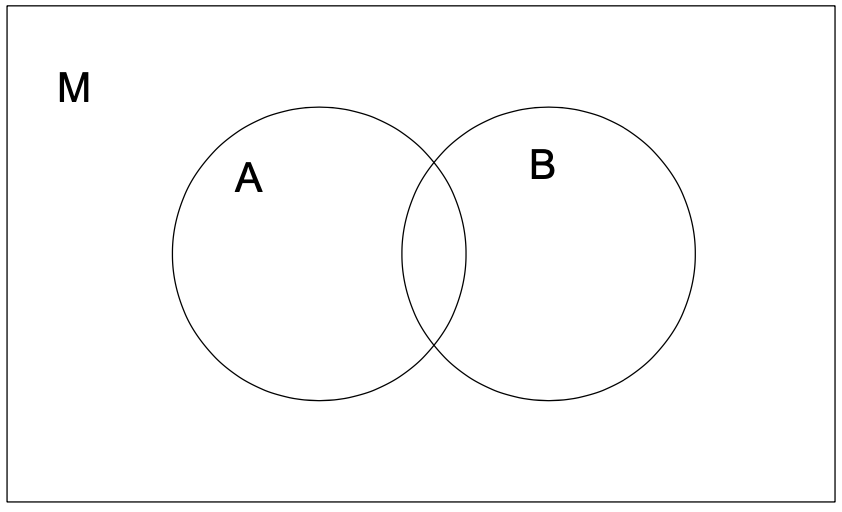
\includegraphics[scale=0.3]{Bilder/venn.png}
	\caption{Darstellung eines Venn Diagramms}
	\end{figure}
	\subsection{Beziehungen zwischen Mengen}
	Um die Beziehung zwischen Mengen darzustellen gibt es mehrere Operationen. Diese sind:
	\subsubsection{Durchschnittsmenge - \texorpdfstring{$\cap$}{}}
	Die Durchschnittsmenge ist die Menge, welche nur in beiden der Mengen vorkommt: $A \cap B = \{x|x \in A \land x \in B \}$ \\
	\begin{center}
	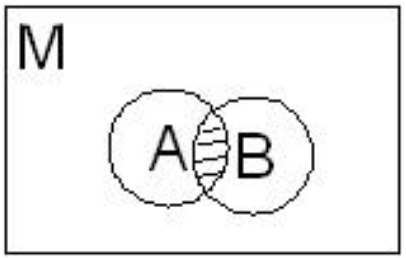
\includegraphics[scale=0.5]{Bilder/durchschnitt.png}
	\end{center}
	\subsubsection{Vereinigungsmenge - \texorpdfstring{$\cup$}{}}
	Die Vereinigungsmenge ist die Menge beider Mengen: $A \cup B = \{x|x \in A \lor x \in B \}$ \\
	\begin{center}
	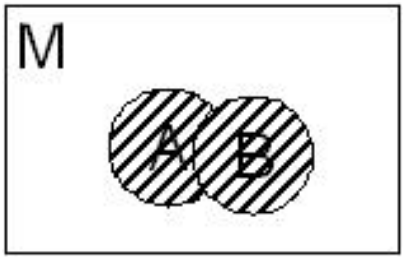
\includegraphics[scale=0.5]{Bilder/vereinigung.png}
	\end{center}
	\subsubsection{Komplementärmenge - \texorpdfstring{$'$}{}}
	Die Komplementärmenge ist die Menge, welche zwar in der Grundmenge M existiert, jedoch nicht in der Menge A: \\
	$A' = \{x|x \in M \land x \notin A \}$ \\
	\begin{center}
	\includegraphics[scale=0.5]{Bilder/komplementär.png}
	\end{center}
	\subsubsection{Differenzmenge - \textbackslash }
	Die Differenzmenge ist die Menge aller Elemente, welche zwar in A enthalten sind, aber nicht in B: A \textbackslash B = $\{x|x \in A \land x \notin B\}$ \\
	\begin{center}
	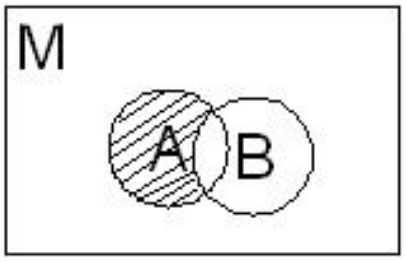
\includegraphics[scale=0.5]{Bilder/differenz.png} \\
	\end{center}
	Zusätzlich gilt, dass wenn B eine Teilmenge von A, so ist A ohne B die Komplementärmenge von B in A: $B \subseteq A:A $\textbackslash$ B = B'$\\
	So kann eine Komplementärmenge angeben, ob sie eine Komplementärmenge einer anderen Menge ist. Wenn nichts angegeben ist, bezieht sich das auf die Grundmenge M.
	\subsection{Mengenoperationen}
	\subsubsection{Disjunkt}	
	Zwei Mengen sind Disjunkt wenn diese keine gemeinsamen Objekte beinhalten: $A \cap B = \{\}$
	\subsubsection{Kartesisches Produkt}
	Das kartesische Produkt (A kreuz B) ist die Produktmenge aller geordneten Paare zweier Mengen A und B: $A x B = \{(a, b)|a \in A \land b \in B\}$\\
	Gesetzmäßigkeit: $A \times B \neq B \times A$ $\to$ Das Kreuzprodukt von A und B ist nicht gleich dem Kreuzprodukt von B und A (Kann aber sein.) \\
	Beispiel: \\
	$\{1,2\}\times\{3,4\} = \{(1,3),(1,4),(2,3),(2,4)\}$ \\
	Also wird jedes Element einer Menge einmal mit jedem Element in der anderen Menge verknüpft.
	\subsubsection{n-faches Produkt}
	Das n-fache Produkt ist einer Erweiterung vom Kartesischen Produkt. Zuvor wurden nur zwei Mengen miteinander verknüpft und jetzt werden n Mengen miteinander verknüpft: $A_1\times A_2 \times A_3 \times ...\times A_n = \{(a_1, a_2, a_3,...,a_n)|a_1 \in A_1, a_2 \in A_2, a_3 \in A_3,...,a_n \in A_n\}$ \\
	Das n-fache Produkt einer Menge A schreibt man: $A\times A\times A\times...\times A = A^n$
	\subsubsection{Zugehörigkeitstafeln}
	Zugehörigkeitstafeln sehen sehr ähnlich zu Wahrheitstabellen aus, zeigen jedoch keine Werte an, sondern geben an, ob ein Element in einer Menge enthalten ist. Bei 1 ist das Element enthalten ($\in$) und bei 0 ist das Element nicht enthalten ($\notin$):\\
	\begin{tabular}{cccccc}
		\toprule
		A & B & A $\cap$ B & A $\cup$ B & A \textbackslash\, B & B \textbackslash\, A \\ \midrule
		0 & 0 & 0 & 0 & 0 & 0 \\ \hline
		0 & 1 & 0 & 1 & 0 & 1 \\ \hline
		1 & 0 & 0 & 1 & 1 & 0 \\ \hline
		1 & 1 & 1 & 1 & 0 & 0 \\
		\bottomrule
	\end{tabular}
	\subsubsection{Rechengesetze für Mengen}
	\begin{itemize}
		\item{Kommutativgesetz}
		\begin{itemize}
			\item{Die Reihenfolge der Mengen spielt zwischen zwei Operatoren keine Rolle.}
			\item{A $\cup$ B = B $\cup$ A}
		\end{itemize}
		\item{Assoziativgesetz}
		\begin{itemize}
			\item{Wenn die Verbindungen die gleichen sind, kann man die Klammern verschieben oder auslassen.}
			\item{(A$\cap$ B)$\cap$ C = A$\cap$ (B$\cap$ C)}
			\item{(A$\cup$ B)$\cup$ C = A$\cup$ (B$\cap$ C)}
		\end{itemize}
		\item{Distributivgesetz}
		\begin{itemize}
			\item{Man kann eine Menge in eine andere verbundene Menge multiplizieren, muss dabei jedoch die Verbindungen umkehren ($\cup$ zu $\cap$ und umgekehrt)}
			\item{A$\cup$ (B$\cap$ C)=(A$\cup$ B) $\cap$ (A$\cup$ C)}
			\item{A$\cap$ (B$\cup$ C)=(A$\cap$ B) $\cup$ (A$\cap$ C)}
		\end{itemize}
		\item{Idempotenz}
		\begin{itemize}
			\item{Eine Vereinigung oder Differenz von sich selbst, ergibt die Menge.}
			\item{A$\cap$ A = A$\cup$ A = A}
		\end{itemize}
		\item{Identität}
		\begin{itemize}
			\item{Die Differenz einer Menge mit der leeren Menge ergibt die leere Menge}
			\item{(A$\cap$ \{\})=\{\}}
			\item{Die Vereinigung einer Menge mit der leeren Menge ergibt die Menge.}
			\item{(A$\cup$ \{\})=A}
		\end{itemize}
		\item{De Morgan'sche Regeln - 1}
		\begin{itemize}
			\item{Die Umkehrung eines Ausdrucks kehrt alle Mengen sowie die Verbindung um ($\cup$ zu $\cap$ und umgekehrt)}
			\item{(A$\cap$ B)'=A'$\cup$ B'}
			\item{(A$\cup$ B)'=A'$\cap$ B'}
		\end{itemize}
		\item{De Morgan'sche Regeln - 2}
		\begin{itemize}
			\item{Das Distributivgesetz funktioniert auch bei der Schnittmenge}
			\item{A\textbackslash (B$\cap$ C)=(A\textbackslash B)$\cup$ (A\textbackslash C)}
			\item{A\textbackslash (B$\cup$ C)=(A\textbackslash B)$\cap$ (A\textbackslash C)}
		\end{itemize}
		\item{Weitere Rechengesetze}
		\begin{itemize}
			\item{}
		\end{itemize}
	\end{itemize}
	\section{Zahlenmengen}
	Zahlenmengen geben die Menge einer spezifischen Zahlenmenge an. Natürliche Zahlen stellen, beispielsweise, nur ganze positive Zahlen dar. Jede dieser Mengen enthält die vorherige Menge komplett.
	\subsection{Natürliche Zahlen - \texorpdfstring{$\N$}{}}
	Die natürlichen Zahlen sind die kleinste Menge und beinhalten nur die ganzen positiven Zahlen. Eine Erweiterung dessen ist $\N_0$, was auch die Null beinhaltet. Die Natürlichen Zahlen sind eine unendliche Menge, wodurch es keine größte Zahl gibt. Daher gibt es zu jeder natürlichen Zahl eine größere Zahl. Jedoch sind sie nach unten begrenzt und somit sind entweder 1 oder 0 die kleinsten Zahlen. Natürliche Zahlen sind geordnet, also gibt es zu jeder Zahl einen eindeutigen Nachfolger. \\
	In den natürlichen Zahlen sind Addition und Miltiplikation uneingeschränkt möglich, also kann man zwei Zahlen aus den natürlichen Zahlen nehmen, diese addieren oder multiplizieren und bekommt stets eine weitere natürliche zahl.
	\subsection{Ganzen Zahlen - \texorpdfstring{$\Z$}{}}
	Die ganzen Zahlen sind alle natürlichen Zahlen inklusive der negativen Zahlen. Die Menge ist wieder unbeschränkt, jedoch nach oben und nach unten, also geht die Menge von negativ unendlich bis positiv unendlich. \\
	Ganze Zahlen haben nun zwei eindeutige Nachbarn, jeweils eine größere und eine kleinere Zahl. Bei den natürlichen Zahlen gab es nur eine eindeutige größere Zahl. \\
	Die Ordnungsrelation der ganzen Zahlen besagt, dass $\forall m, n \in \Z : m<n \iff -m > -n$, also sind, wenn eine Zahl größer ist als die andere, die negativen Äquivalente davon auch größer als die andere. \\
	Hier sind nun Division, Addition und Multiplikation uneingeschränkt möglich, also kann man jede ganze Zahl von jeder anderen Zahl addieren, multiplizieren oder subtrahieren und erhält eine weitere ganze Zahl.
	\subsection{Rationale Zahlen - \texorpdfstring{$\Q$}{}}
	Zur Verwendung von Division benötigt man die rationalen Zahlen. Diese sind definiert als alle möglichen Brüche $\frac{p}{q}$, wobei$p,q \in \Z und q \neq 0$. Hier kann man alle Grundrechnungsarten verwenden.
	\subsubsection{Rechenregeln rationaler Zahlen}
	\begin{itemize}
		\item{Gleichheit:}
		\begin{itemize}
			\item{$\frac{p_1}{q_1}$ = $\frac{p_2}{q_2} \iff p_1q_2 = p_2q_1$}
		\end{itemize}
		\item{Addition}
		\begin{itemize}
			\item{$\frac{p_1}{q1}$ + $\frac{p_2}{q2}$ = $\frac{p_1q_2+p_2q_1}{q_1q_2}$}
		\end{itemize}
		\item{Potenzen}
		\begin{itemize}
			\item{$a^n = a*a*a*a*...*a$}
			\item{Bei negativen Potenzen, wenn $a \neq 0: a^{-n} = \frac{1}{a^n}$}
		\end{itemize}
	\end{itemize}
	Wenn man einen rationalen Exponenten hat, muss die Basis größer gleich 0 sein, also ist die Rechnung $-2^1,7$ nicht definiert. Gleichzeitig muss die Basis größer als 0 sein, wenn der Exponent einen rationale negative Zahl ist.
	\subsubsection{Beweis}
	Dass nicht alle Zahlen mithilfe von rationalen Zahlen dargestellt werden können, kann man mithilfe eines indirekten Beweises belegen. \hyperref[sec:Mathematische Beweise]{\underline{Siehe Beweise}} \\ 
	Der Satz von Euklid besagt, dass es keine rationale Zahl gibt, mit der man $\sqrt{2}$ darstellen kann. Das wird mittels eines indirekten Beweises bewiesen. Dabei wird durch Widerspruch der Verneinung bewiesen, dass die Aussage falsch ist. Also behauptet man zuerst, dass die Annahme falsch ist und beweist danach, dass das zu einem Widerspruch führt. \\
	Die Aussage ist, dass es keine rationale Zahl zur Darstellung von $\sqrt{2}$ gibt: $(\frac{p}{q})^2 = 2$. Dabei dürfen p und q nicht beide gerade Zahlen sein, sonst könnte man sie so weit kürzen, dass diese keine geraden Zahlen mehr sind. \\
	$\frac{p^2}{q^2} = 2$ $\to$ Klammer auflösen |$q^2$ \\
	$p^2 = 2q^2$ $\to$ p ist gerade, da das Quadrat durch 2 teilbar ist. Daher ist eine Zahl durch 2 teilbar, wenn das Quadrat durch 2 teilbar ist. \\
	Aus diesem Grund kann man angeben, dass $p = 2*p_0$ und wenn man dies quadriert erhält man $p^2 = 4*p_0^2$. Aus diesem Grund kann man angeben, dass $4*p_0^2 = 2q^2$. \\
	Wenn man dies nun kürzt erhält man: $2p_0^2 = q^2$. Da wir wissen, dass p gerade ist, weil das Quadrat durch $q^2$ durch 2 teilbar ist, müssen wir nun annehmen, dass q auch gerade ist, da nun impliziert wird, dass beide Zahlen gerade sind. Jedoch wurde Anfangs definiert, dass beide Zahlen nicht gerade sein dürfen. Das ist ein Widerspruch und beweist, dass die ursprüngliche Aussage nicht wahr sein kann $\to$ q.e.d.
	\subsection{Reelle Zahlen - \texorpdfstring{$\R$}{}}
	Reelle Zahlen beinhalten alle Zahlen, jedoch auch irrationale Zahlen, welche unendliche, nicht periodische Dezimalbrüche haben. Diese Zahlen haben eine sich nicht feststellbare wiederholende Ziffernfolge. \\ 
	Beispiele für reelle Zahlen sind: \\
	$\sqrt{2}=1,41421356$ \\
	$Eulersche Zahl\ e=2,718281828$ \\
	$Kreiszahl\ \pi = 3,14159$
	\subsubsection{Intervalle}
	Intervalle sind eine andere Art der Mengenangabe: \\
	$[a,b] = \{x\in \R | a \leq x \leq b\}$ - Abgeschlossenes Intervall $\to$ Ein Intervall von a bis b, inklusive a und b \\
	$(a,b] = \{x \in \R | a < x \leq b \}$ - Halboffenes Intervall von a $\to$ Ein Intervall von a bis b, ohne a \\
	$[a,b) = \{x\in \R | a \leq x < b \}$ - Halboffenes Intervall von b $\to$ Ein Intervall von a bis b, ohne b \\
	$(a,b) = \{x \in \R | a < x < b \}$ - Geschlossenes Intervall - Ein Intervall von a bis b ohne a oder b \\
	Intervalle haben immer eine unendliche Mächtigkeit, da diese immer Teil der reellen Zahlen sind.
	\subsubsection{Schranken}
	Schranken beschränken die Größe einer Menge. Die kleinste obere Schranke nennt man \textbf{Supremum}. Wenn dieses Teil der Menge ist, wird es \textbf{Maximum} genannt.\\
	Das gleiche gilt für die unteren Schranken wobei man diese \textbf{Infimum} nennt. Wenn es Teil der Menge ist, nennt man sie \textbf{Minimum}. \\
	Dabei gilt jedoch, dass falls die Schranke nicht Teil der Menge ist, ist das Maximum und Minimum nicht definiert, da man dann stets eine weitere Kommastelle hinzufügen kann.
	\subsection{Komplexe Zahlen - \texorpdfstring{$\mathbb{C}$}{}}
	Komplexe Zahlen erweitern reelle Zahlen um eine imaginäre Einheit \textit{i}. Diese Zahlen haben den Sonderfall, dass die imaginäre Einheit $i^2$ gleich -1 ergibt. Dadurch ergibt sich auch, dass \textit{i} die Wurzel von -1 hat. Jede imaginäre Zahl hat somit einen Realteil und Imaginärteil. Komplexe Zahlen werden in der Elektrotechnik und der Signalverarbeitung verwendet.
	\section{Summen und Produkte}
	\subsection{Summen}
	Summen geben eine kontinuierliche Summierung einer Reihe an. \\
	$\sum_k=1^na_k = a_1+a_2+a_3+...+a_n$ - Wobei k die Laufvariable ist, welche stets erhöht wird. 1 ist der Startwert oder die untere Grenze. n stellt den Endwert oder die obere Grenze dar. $a_k$ beschreibt dabei die Funktion, welche summiert wird. \\
	Summenrechenregeln sind:
	\begin{itemize}
		\item{$\sum_{k=0}^{n}(a_k+b_k)=\sum_{k=0}^{n}a_k+\sum_{k=0}^{n}b_k$}
		\begin{itemize}
			\item{Man kann, wenn eine Addition innerhalb einer Summe vorhanden ist, diese in zwei separate Summen aufspalten.}
		\end{itemize}
		\item{$\sum_{k=0}^{n}c*a_k=c*\sum_k=0^na_k$}
		\begin{itemize}
			\item{Man kann, wenn eine Multiplikation innerhalb einer Summer vorhanden ist, die Multiplikation vor das Summensymbol stellen und sie so aufteilen.}
		\end{itemize}
	\end{itemize}
	\subsection{Produkte}
	Das selbe Prinzip existiert auch bei kontinuierlicher Multiplikation: \\
	$\prod_{k=1}^{n} a_k = a_1 * a_2 * a_3 * ... * a_n$ Wobei die gleichen Parameter wie bei der Summe bestehen.
	\section{Mathematische Beweise}
	\label{sec:Mathematische Beweise}
	Da die Mathematik grundsätzlich aus Aussagen und Sätzen besteht, müssen diese auch bewiesen werden. Es gibt mehrere Beweisführungsarten:
	\subsection{Direkter Beweis}
	Der direkte Beweis stützt seine Aussage auf eine bereits bewiesene wahre Aussage. $v_1 \implies v_2 \implies ... \implies a$ ist wahr. \\
	Ein Beispiel ist der Beweis, dass das Quadrat jeder geraden natürlichen Zahl auch gerade ist. Dabei beginnt man den Beweis indem man Definitionen am Anfang und Ende auflöst um danach die Lücken zu schließen:
	\begin{enumerate}
		\item{Behauptung: Wenn $x$ eine natürliche gerade Zahl ist, dann gilt: $x = 2y$}
		\item{Erster Schritt wäre, davon das Quadrat zu bilden: $x^2 = (2y)^2 = 4y^2$}
		\item{$x^2 = 4y^2 \to 2(2y^2) \to 2z$}
		\item{Ende: $x^2 = 2z$}
	\end{enumerate}
	Ein weiteres Beispiel ist der Beweis, dass a+b halbe, stets mehr oder gleich viel ist, als die Wurzel von a mal b: \\
	\begin{enumerate}
		\item{$a,b \in\R; a \geq 0, b\geq 0: \frac{a+b}{2} \geq \sqrt{a*b}$}
		\item{Behauptung: $\frac{a+b}{2} \geq \sqrt{a*b}$}
		\item{Beweis: $(a-b)^2 \geq 0$ $\to$ Zweite binomische Formel.}
		\item{$(a^2-2ab+b^2)\geq 0 \to$ Quadrat auflösen}
		\item{$(a^2+2ab+b^2)\geq 4ab \to 4ab$ addieren um die erste binomische Formel zu formen.}
		\item{$(a+b)^2 \geq 4ab \to$ Erste binomische Formel generieren.}
		\item{$\frac{(a+b)^2}{4} \geq ab$ $\to$ Durch 4 dividieren}
		\item{$\sqrt{\frac{(a+b)^2{4}}\geq \sqrt{ab}}$ $\to$ Wurzel ziehen}
		\item{$\frac{a+b}{\sqrt{4}}\geq \sqrt{ab}$ $\to$ Wurzel beider Teile ziehen}
		\item{$\frac{a+b}{2}\geq \sqrt{ab}$}
	\end{enumerate}
	\subsection{Indirekter Beweis}
	Der indirekte Beweis behauptet stattdessen, dass die falsche Behauptung wahr ist, um danach zu beweisen, dass dessen Widerspruch bedeutet, dass die Behauptung wahr ist. \\
	Beispiel: Keine ganze Zahl ist gerade und ungerade zugleich. \\
	Die Verneinung dieser Behauptung ist, dass ein \textit{x} existiert, welches gerade und ungerade zugleich ist. \\
	\begin{itemize}
		\item{Wenn \textit{x} gerade ist, gibt es eine Zahl \textit{a}, sodass $x=2a$}
		\item{Wenn \textit{x} ungerade ist, gibt es eine Zahl \textit{b}, sodass $x=2b+1$}
	\end{itemize}
	Da \textit{x} gerade und ungerade zugleich ist, sind beide dieser Behauptungen wahr und man kann diese gleichsetzen: \\
	$2a = 2b + 1$ \\
	Dividiert man beide Seiten durch 2, so ergibt sich $a = b + \frac{1}{2}$ und bei weiterer Umformung $ a - b = \frac{1}{2}$\\
	Da a und b ganze Zahlen sind, sollte die Subtraktion dessen zu einer weiteren ganzen Zahl und nicht zu einer rationalen Zahl führen.
	\paragraphlb{Beispiel:}
	Vorraussetzungen: \\
	$a,b \in\R, a\geq0, b\geq0$ \\
	$(a-b)^2\geq 0\ \forall a,b\in\R$ \\
	Behauptung: $\frac{a+b}{2} \geq \sqrt{a*b}$
	\begin{enumerate}
		\item{Verneinung der Behauptung: $\frac{a+b}{2} < \sqrt{a*b}$}
		\item{$a+b < 2*\sqrt{a*b}$ $\to$ Multiplikation mit 2}
		\item{$(a+b)^2 < 4*ab$ $\to$ Quadrierung}
		\item{$a^2+2ab+b^2<4ab$ $\to$ Erste binomische Formel}
		\item{$a^2-2ab+b^2 < 0$ $\to$ -4ab}
		\item{$(a-b)^2 < 0$ $\to$ Zweite Binomische Formel}
		\item{Da festgehalten wurde, dass $(a-b)^2$ stets größer oder gleich als null ist, haben wir einen Widerspruch.}
	\end{enumerate}
	\subsection{Gegenbeispiele:}
	Bei Gegenbeispielen muss man keine Beweisführung aufbauen sondern lediglich mit Gegenbeispielen beweisen, dass die Aussage falsch ist. Das ist möglich in Fällen, in welchen ein Beispiel, welches der Regel nicht entspricht, dieses widerlegt.
	\paragraphlb{Beispiel:}
	Behauptung: $3x+7<12$ gilt für alle $x\in\N_0$. \\
	Beweis: \\
	x = 0 $\to$ $3*0+7<12$ $\to$ Wahr \\
	x = 1 $\to$ $3*1+7<12$ $\to$ Wahr \\
	x = 2 $\to$ $3*2+7<12$ $\to$ Falsch \\
	Deshalb gilt die Ungleichung nicht für alle $x\in \N_0$
	\subsection{Vollständige Induktion}
	Bei der vollständigen Induktion wird bewiesen, dass eine Aussage für alle natürlichen Zahlen wahr ist. Da man es nie manuell für alle natürlichen Zahlen beweisen kann, muss man stattdessen beweisen, dass es für eine Zahl gilt und auch für dessen Nachfolger.
	\paragraphlb{Beispiel:}
	Zeigen Sie, dass $3^{2n+4}-2^{n-1}$ durch 7 teilbar ist. Dabei muss man zuerst den Anfang definieren, welcher normalerweise die kleinste mögliche Zahl ist: \\
	\begin{enumerate}
		\item{Anfang: $n_0=1: 3^{2*1+4}-2^{1-1}=728\to 7*104$}
		\item{Vorraussetzung: $n\in\N: 3^{2n+4}-2^{n-1}=7*p, p\in\N$. p nimmt hierbei das Ergebnis ein, welches durch 7 teilbar ist.}
		\item{Behauptung: $3^{2(n+1)+4}-2^{(n+1)-1} = 7*m, m\in\N$. Da der nächste Wert ein anderer sein wird, nimmt das Ergebnis auch eine neue Variable an.}
		\item{Beweis: $3^{2(n+1)+4}-2^{(n+1)-1}$}
		\item{$3^{2n+2+4}-2{n}\ \to 3^{2n+4+2}-2^n$}
		\item{$3^{2n+4}*3^2-2^n$}
		\item{$3^{2n+4}*9-2^n$}
		\item{Nebenrechnung: Umformung der Vorraussetzung: $3^{2n+4}-2^{n-1} = 7p \to 3^{2n+4} = 7p+2^{n-1}$. Da dieser Term der gleiche wie der in der Beweislage ist, kann man diesen ersetzen.}
		\item{$(7p+2^{n-1})*9-2^n$}
		\item{$7*9p+9*2^{n-1}-2^n \to$ Herausmultiplizieren}
		\item{$7*9p+(9-2)*2^{n-1} \to$ $2^{n-1}$ herausheben da $2^{n-1}*2^1 = 2^n$}
		\item{$7*9p + 7*2^{n-1}$}
		\item{$7(9p+2^{n-1}) \to$ Herausheben von 7, da es Teil von beiden Werten ist.}
		\item{Da sowohl p als auch n Teil der natürlichen Zahlen sind, bedeutet das, dass dieser Term gleichbedeutend mit $7*m$ ist.}
	\end{enumerate}
	\paragraphlb{$\sum^n_{k=1}{k}=\frac{n(n+1)}{2}$}
	Zeigen Sie, dass die Summer aller natürlichen Zahlen $\sum^n_{k=1}{k}$ gleich $\frac{n(n+1)}{2}$ ist. \\
	1. Induktionsanfang: n=1 $\sum^{1}_{k=1}{k} = 1 \to \frac{1(1+1)}{2} = 1$ \\
	Grundlegend wurde festgestellt, dass für das kleinstmögliche n (In diesem Fall 1) die Aussage wahr ist. \\
	2. Induktionsvorraussetzung: $n\in \N:\sum^{n}_{k=1}{k}=\frac{n(n+1)}{2}$ \\
	3. Behauptung: $\sum^{n+1}_{k=1}{k}=\frac{(n+1)((n+1)+1)}{2}=\frac{(n+1)(n+2)}{2}=\frac{n^2+3n+2}{2}$ \\
	Nun wurde jedes n durch ein ein n+1 ersetzt und vereinfacht. \\
	4. Beweis: $\sum^{n+1}_{k=1}{k}=\sum^{n}_{k=1}{k} \to$ Wir stützen uns auf die frühere Summe, müssen diese jedoch um 1 erhöhen: \\
	$\sum^{n+1}_{k=1}{k}=\sum^{n}_{k=1}{k+(n+1)} \to$ Also muss, um die Formel gleichzusetzen jeweils das n um 1 erhöht hinzugefügt werden. \\
	Jetzt kann man erneut die anfängliche Behauptung aufstellen: $\sum^{n}_{k=1}{k+(n+1)} = \frac{n(n+1)}{2}+(n+1)$ \\
	Nun sollte das n+1 des rechten Terms in den Bruch integriert werden. Dazu muss man, da der Bruch durch 2 geteilt wird, diesen auch mit 2 multiplizieren $\to \frac{n(n+1)+2(n+1)}{2}=\frac{n^2+n+2n+2}{2}=\frac{n^2+3n+2}{2}$
	\paragraphlb{$\sum^{n}_{i=1}{\frac{1}{(3i-2)(ei+1)}}=\frac{n}{3n+1}$}
	1. Anfang: n=1 $\sum^{n}_{i=1}{\frac{1}{(3i-2)(ei+1)}}=\frac{1}{3*1-2}{3*1+1}=\nicefrac{1}{4}$ - $\frac{1}{3*1+1}=\nicefrac{1}{4}$ \\
	2. Vorraussetzung: $n\in\N:\sum^{n}_{i=1}{\frac{1}{(3i-2)(3i+1)}}=\frac{n}{3n+1}$ \\
	3. Behauptung: $\sum^{n+1}_{i=1}{\frac{1}{(3i-2)(3i+1)}}=\frac{n+1}{3(n+1)+1}=\frac{n+1}{3n+4}$ \\
	4. Beweis: $\sum^{n+1}_{i=1}{\frac{1}{(3i-2)(3i+1)}}=\sum^{n}_{i=1}{\frac{1}{(3i-2)(3i+1)}}+\frac{1}{(3(n+1)-2)(3(n+1)+1)} \to$ Da der Term innerhalb der Summe steht, muss man den gesamten Term duplizieren um ihn so mit dem linken Term gleichzusetzen. \\
	$\sum^{n}_{i=1}{\frac{1}{3i-2)(3i+1)}}+\frac{1}{(3n+3-2)(3n+3+1)} = \frac{n}{3n+1}+\frac{1}{(3n+1)(3n+4)} = \frac{n(3n+4)+1}{(3n+1)(3n+4)}=\frac{3n^2+4n+1}{(3n+1)(3n+4)}$\\
	Da in dem rechten Term der Behauptung unter dem Bruch ein 3n+4 steht, sollte man versuchen es dorthin zu vereinfachen. Dazu muss man jedoch die Polynomfunktion auflösen. Dafür gibt es drei Strategien:
	\begin{itemize}
		\item{Polynomdivision - Verringerung des Polynoms um einen Faktor}
		\item{Polynomfaktorisierung - Linerafaktorzerlegung durch Einfügen der kleinen Formel.}
		\begin{itemize}
			\item{$3n^2+4n+1 = 0 \to n_{1,2}=\frac{-b\pm\sqrt{b^2-4ac}}{2a} = \frac{-4\pm\sqrt{4^2-4*3}}{2*3} = \frac{-4\pm2}{6} \to n_1 = -1/n_2 \to \nicefrac{1}{3}$}
			\item{Man kann die Ergebnise dieser Formel anders darstellen um sie auszurechnen: $(n-n_1)(n-n_2)...(n-n_n)$}
			\item{Also kann man das Ergebnis so aufschreiben: $3*(n+\nicefrac{1}{3})(n+1)=(3n+1)(n+1)$}
		\end{itemize}
		\item{Intuition - Ungefähr abschätzen in welche Faktoren es zu zerlegen ist un diese verwenden.}
	\end{itemize}
	Da man hoffentlich (3n+1) kürzen kann, um den gewünschten Bruch zu erreichen, kann man den ersten Term nun verwenden $\to$ $\frac{3n^2+4n+1}{(3n+1)}=\frac{(3n+1)(n+1)}{(3n+1)(3n+4)}$ $\to$ Man ersetzt das Ergebnis der Polynomfunktion durch das Ergebnis und erhält so eine kürzbare Formel $\to$ = $\frac{n+1}{3n+4}$
	\paragraphlb{$2^n > n^2$ für alle $n \geq 5$}
	1. Anfang: n=5: $2^5=32 > 5^2 = 25$ \\
	2. Vorraussetzung: $n\in\N, n\geq 5:2^n>n^2$\\
	3. Behauptung: $2^{n+1} > (n+1)^2=(n+1)(n+1) = n^2+2n+1$ \\
	4. Beweis: $2^{n+1} = 2^n * 2^1 > n^2*2$ $\to$ Man will diese Formel nun der Behauptung gleichsetzen. Da es sich jedoch um eine Ungleichung handelt, muss man diese Verändern. Da wir eine Ungleichung haben, in welcher der rechte Term kleiner ist als der linke, bedeutet das, dass man jeweils den linken Term vergrößern oder den rechten Term verkleinern, ohne die Gültigkeit der Gleichung zu gefährden. \\
	Da wir durch Einsetzen wissen, dass der Term zu groß ist, verkleinern wir den rechten Term um ihn hoffentlich anzupassen $\to$ $> n^2 + n^2 = n^2+n*n$. \\
	Eines dieser ns kann man nun durch einen Wert ersetzen $\to$ $n^2+3*n = n^2+2n+n$ $\to$ Da man auch noch eine 1 benötigt, kann man für eines der ns jetzt noch durch 1 ersetzen um zu der gesuchten Formel zu kommen $\to$ $n^2+2n+1$ \\
	Dieser Rechenvorgang ist möglich, weil man den Wert des kleineren Teils der Ungleichung beliebig verkleinern und den größeren Teil der Ungleichung beliebig vergrößern kann und die Ungleichung behält trotzdem ihre Gültigkeit. Man sollte jedoch bedenken, dass dieser Vorgang nur möglich ist, solange der ersetzte Wert kleiner oder gleich groß, als der kleinstmögliche Wert von n ist.
	\paragraphlb{$2^n > n^3$ für alle $n \geq 10$}
	1. Anfang: n=10 $2^10 = 1024 > 10^3 = 1000$ $\to$ Korrekt \\
	2. Vorraussetzung: $n\in\N, n\geq10:2^n>n^3$ \\
	3. Behauptung: $2^n+1>(n+1)^3 = (n+1)(n+1)(n+1)=n^3+3n^2+3n+1$ \\
	4. Beweis: $2^{n+1}=2^n*2 > n^3*2$ $\to$ $n^3 + n^3 = n^3 + n*n^2$ $\to$ Man benötigt einige Terme um den richtigen zu konstruieren. Aus diesem Grund sollte man den Term n durch einen Wert, welcher garantiert kleiner als n ist, ersetzen (Also kleiner oder gleich 10) $\to$ $> n^3 +10n^2 = n^3+3n^2+3n^2+4n^2$ $\to$ $n^3+3n^2+3n*n+4n^2$ $\to$ $n^3+3n^2+3n+1$ $\to$ Im letzten Fall kann man den Term $4n^2$ durch 1 ersetzen, da, wenn n größer oder gleich 10 ist, ist es definitiv größer als 1.
	\section{Teilbarkeit und Primzahlen}
	Eine Zahl gilt als teilbar, wenn eine natürliche Zahl \textit{b} und eine andere natürliche Zahl \textit{a} durch $a=n*b$ darstellbar ist. Das kann man auch als $a|b$ darstellen. \\
	Grundsätzlich ist jede Zahl durch 1 und sich selbst teilbar. Ein Teiler \textbf{ist immer positiv.} \\
	Wenn man also die Zahl 15 nimmt, kann man dies durch $1*15 = 15$ und $15 = 3*5$ darstellbar. Dadurch sind die Teiler von 15, 1, 3, 5 und 15. Dasselbe gilt auch falls 15 negativ ist, also sind die Teiler von -15 auch 1, 3, 5 und 15.
	\subsection{Primzahlen}
	Eine Zahl ist eine Primzahl, wenn sie größer als 1 ist und nur durch 1 und sicht selbst teilbar ist. Zum Beispiel sind 2, 3, 5 und 7 Primzahlen. 4 ist hierbei keine Primzahl, da sie durch $2*2$ darstellbar ist.
	\subsubsection{Primfaktorzerlegung}
	Jede Zahl ist entweder eine Primzahl oder lässt sich als Produkt von Primzahlen darstellen. Diese Faktoren sind außer in der Reihenfolge eindeutig. Dabei nennt man diese Sequenz an Faktoren \textbf{Primfaktoren.} Beispiele von Primfaktorzerlegung sind:\\
	$4=2*2$ \\
	$30=2*3*5$ \\
	Der Weg zur Ermittlung der Primfaktoren ist, eine Zahl durch jede Primzahl aufsteigend zu dividieren:\\
	\begin{tabular}{ c | c }
	 	30 & 2 \\
	 	15 & 3 \\
	 	5 & 5 \\
	 	1 & 1 \\
	 \end{tabular}  \\
	 Hier wird zuerst durch 2 dividiert, das Ergebnis durch 3 geteilt und dessen Ergebnis wieder durch 5 geteilt. Da 1 keine Primzahl ist, wird es ausgelassen. Somit sind die Primfaktoren von 30, 2, 3 und 5.
	 \subsection{Größter gemeinsamer Teiler (ggT)}
	 Der größte gemeinsame Teiler zweier Zahlen ist der größte Wert, welcher durch beide Zahlen teilbar ist. Man kann den ggT ermitteln, indem man die Primfaktorzerlegung bei beiden Zahlen anwendet und den größten Primfaktor wählt.
	 \subsection{Kleinstes gemeinsames Vielfaches (kgV)}
	 Das kleinste gemeinsame Vielfache zweier Zahlen ist die kleinste Ganzzahl, welche mit zwei Zahlen multipliziert werden könnnen. Diese erhält man, indem man wiederum die Primfaktorzerlegung anwendet und jeden Primfaktor, welcher mindestens einmal vorkommt miteinander multipliziert.
	 \subsection{Teilerfremde Zahlen}
	 Zwei Zahlen gelten als teilerfremd, wenn sie keinen gemeinsamen Primfaktor haben. Man kann dies wiederum ermitteln indem man bei beiden Zahlen eine Primfaktorzerlegung anwendet und überprüft, ob sie mindestens einen Primfaktor gemeinsam haben.
	 \subsection{Division mit Rest}
	 Wenn zwei Zahlen nicht teilbar sind, dann bleibt ein Rest. Dies wird definiert durch $a=q*m+r mit 0\geq m$. Also stellt es eine Multiplikation mit einem hinzugefügten Wert dar. Die mathematischen Schreibweisen sind: \\
	 $17\ mod\ 5$ und $17\ div\ 5$. div ist hierbei die Ganzzahldivision und hinterlässt keinen Rest.
	 \subsubsection{Modulo bei negativen Zahlen}
	 Laut Definition darf der Rest nicht kleiner als 0 sein. Falls a kleiner als 0 ist muss man m zum negativen Rest hinzuaddieren. Wenn man also $-17\ div\ 5=-3, -2\ Rest$ erhält, muss man 5 erneut zu dem Rest addieren, $-2+5=3$. Da dies jedoch zu einer inkorrekten Formel $-17=-3*5+3$ führen würde, muss man das Ergebnis um 1 erhöhen (bzw. verringern) $\to$ $-17=-4*5+3$. \\
	 \section{Relationen}
	 Relationen helfen die Beziehung zwischen zwei Objekten oder Mengen zu beschreiben. Diese können Personen, Gegenstände, Zahlen aber auch allgemeine Objekte sein. Eine mögliche Relation ist kleiner-als (<). Wenn man diese für natürliche Zahlen definiert, gibt es Zahlenpaare welche der Relation genügen. Zum Beispiel (2, 8) (Da 2 kleiner ist als 8). Jedoch gibt es auch Paare, welche nicht genügen wie (10, 3) (Da 10 größer ist als 3). \\
	 Bei einer Relation kann man auch zwei Mengen in relation stellen. Wenn man zum Beispiel eine Menge von Städen (Berlin, Wien, Bern) und die Menge aller Länder Europas nimmt, wobei die Relation \verb|Stadt liegt in Land| besteht, dann gibt es genau drei Paare, da jede Stadt nur in einem Land sein kann. \\
	 Eine Relation ist also eine Menge aus geordneten Paaren: $(x,y)\in\R\iff xRy$, auch geschrieben als a$\sim$ b. Dabei gilt zusätzlich, dass eine Relation einer Menge, auch eine Teilmenge dessen kartesischen Produkts ist: $A\times A, R \subseteq A\times A$. \\
	 Ein Unterschied zur mathematischen Funktion ist, dass ein Element aus einer Menge mehrmals aber auch gar nicht in einer Relation vorkommen kann. In einer Funktion kann ein x beispielsweise nur ein y haben. \\
	 Wenn man zum Beispiel eine Menge aus Städten und Bundesländern hat, kann es passieren, dass zwei Städte im selben Bundesland liegen, aber auch, dass die Stadt in keinem der Bundesländer der Menge liegt.
	 \subsection{Umkehrrelation}
	 Die inverse Relation oder Umkehrrelation einer Relation $R$ schreibt man $R^{-1}$. Dabei wird die Reihenfolge aller geordneten Paare gebildet: $R=\{(1,5),(1,4),(1,3)\}$ und $R^{-1}=\{(5,1),(4,1),(3,1)\}$. Diese Umkehrung ist bei Zahlen relativ simpel. Falls die Relation jedoch eine Aussage wie \textit{A ist Kind von B} ist, dann ist die Umkehrrelation \textit{A ist Elternteil von B}. \\
	 Beispiel: Kehren sie folgende Relation um:
	 $R=\{(a,c),(b,a),(b,b),(b,c),(d,d)\}\ \to R^{-1} = \{(c,a),(a,b),(b,b),(c,b),(d,d)\}$ \\
	 \subsection{Verknüpfung von Relationen}
	 Man kann aus Relationen auch neue Relationen bilden: $R\subseteq A\times B$ und $S\subseteq B\times C$. Die Verbindung zweier Relationen nennt man Verknüpfung. Eine solche Verknüpfung schreibt man $S°R$, was "S nach R" genannt wird. Dabei werden die Bezeichnungen der Mengen vertauscht. Also wird bei der Verknüpfung der Relationen R und S danach S°R geschrieben. Solche Verknüpfungen sind dadurch auch nicht kommutativ also gilt $S°R \neq R°S$. Ein Beispiel einer Verknüpfung sind die Relationen "ist-Mutter-von" und "ist-verheiratet-mit". Die Verknüpfung dieser Relationen würde danach "ist-Schwiegermutter-von" lauten. \\
	 Ein weiteres Beispiel sind die Mengen: $A=\{1,2,3\}, B=\{a,b,c\}, C=\{x,y,z\}$. Die Relationen dieser Mengen sind: $R=\{(1,a),(2,b),(3,c)\}$ und $S=\{(a,x),(a,y),(b,z)\}$ $\to$ $S°R=\{(1,x),(1,y),(2,z)\}$ wobei es für (3,c) kein Paar gibt. Also wird stets ein Element aus beiden Relationen genommen. Dabei muss der linke Wert der ersten Relation mit der rechten der zweiten Relation übereinstimmen, oder umgekehrt. $\to$ $(a,c)$ und $(c,a)$ $\to$ $(a,a)$ 
	 \subsection{Eigenschaften von Relationen}
	 Relationen haben mehrere Eigenschaften:
	 \begin{itemize}
	 	\item{Reflexiv - $xRx$}
	 	\begin{itemize}
	 		\item{$\forall x\in A:(x,x)\in R$ $\to$ Für alle x der natürlichen Zahlen gilt, dass sie  in Relation zu sich selbst stehen.}
	 		\item{Eine Relation ist genau dann relfexiv wenn alle Paare in Relation zu sich selbst stehen. Dabei könenn auch andere Paare vorkommen, solange jedes der Elemente innerhalb der Relation in Relation zu sich selbst steht.}
	 	\end{itemize}
	 	\item{Irreflexiv - $\neg (xRx)$}
	 	\begin{itemize}
	 		\item{$\forall x\in A:(x,x)\notin R$ $\to$ Für alle x der natürlichen Zahlen gilt, dass keines der Elemente in Relation zu sich selbst stehen.}
	 		\item{Eine Relation ist dann irreflexiv wenn keines der Paare in Relation zu sich selbst stehen.}
	 	\end{itemize}
	 	\item{Identitätsrelation}
	 	\begin{itemize}
	 		\item{$I_A=\{(a,a)|a\in A\}$ $\to$ Eine striktere Reflexivität. Eine Relation ist eine Identitsärelation wenn alle Elemente der Relation nur in Relation zu sich selbst stehen. Dadurch ist eine Identitätsrelation auch gleichzeitig reflexiv.}
	 	\end{itemize}
	 \end{itemize}
	 Wenn man also die Menge $A=\{1,2,3\}$ mit der Relation R auf A hat: \\
	 $R=\{(1,3),(2,2),(3,2),(1,1),(3,3)\}$ $\to$ Reflexiv: Jedes der Mengenelemente hat eine Relation mit sich selbst.\\
	 $R=\{(1,2),(1,3),(2,1)\}$ $\to$ Irreflexiv: Keines der Mengenelemente hat eine Relation mit sich selbst.\\
	 $R=\{(1,3),(2,3),(3,3)\}$ $\to$ Weder noch: Eines der Mengenelemente hat eine Relation mit sich selbst, aber nicht alle.\\
	 \begin{itemize}
	 	\item{Symmetrisch - $xRy \implies yRx$}
	 	\begin{itemize}
	 		\item{$\forall x,y\in A:(x,y)\in R \implies (y,x)\in R$ $\to$ Es muss von jedem Paar auch ein gespiegeltes Paar vorkommen.}
	 	\end{itemize}
	 	\item{Asymmetrisch - $xRy \implies \neg (yRx)$}
	 	\begin{itemize}
	 		\item{$\forall x,y\in A:(x,y)\in R \implies\ (y,x) \notin R$ $\to$ Keines der Paare darf eine Spiegelung eines anderen Paares sein. Es kann dadurch kein Paar geben, welches in Relation zu sich selbst stehen z.B. (1,1)}
	 	\end{itemize}
	 	\item{Antisymmetrisch - $xRy \land yRx \implies x = y$}
	 	\begin{itemize}
	 		\item{$\forall x,y\in A:(x,y)\in R \land (y,x)\in R \implies\ x = y$ $\to$ Alle gespiegelten Paare haben die gleichen Werte. Sobald eines der Paare gespiegelt und ungleich ist, ist es nicht antisymmetrisch.}
	 	\end{itemize}
	 	\item{Relationen $\to$ Asymmetrisch/Antisymmetrisch}
		\begin{itemize}
	 		\item{Der Unterschied zwischen asymmetrisch und antisymmetrisch ist die asymmetrische Relation R: $R^{-1} \cap R = \{\}$ $\to$ Eine Relation ist asymmetrisch wenn die Umkehrrelation geschnitten mit der Relation R die leere Menge bildet.}
	 		\item{Antisymmetrische Relation R: $R^{-1} \cap R \subseteq I_A$(Identitätsrelation) $\to$ Eine Relation ist antisymmetrisch wenn man die Umkehrrelation mit der Relation R schneidet und dadurch eine Identitätsrelation erhält.}
	 		\item{$asymmetrisch \implies\ antisymmetrisch$ $\to$ Jede asymmetrische Relation ist auch gleichzeitig antisymmetrisch (aber nicht umgekehrt)}
		\end{itemize}
	 \end{itemize}
	 Wenn man also wieder die Menge $A=\{1,2,3\}$ mit der Relation R auf A hat: \\
	 $R=\{(1,1),(1,2),(2,1),(3,3)\}$ $\to$ Symmetrisch: Alle Paare haben ein gespiegeltes Gegenstück. \\
	 $R=\{(1,2),(1,3),(2,3)\}$ $\to$ asymmetrisch und antisymmetrisch: Keines der Paare hat ein gespiegeltes Gegenstück wodurch auch alle gespiegelten Paare ein Gegenstück haben.
	 \begin{itemize}
	 	\item{Transitiv - $xRy \land yRz \implies xRz$}
	 	\begin{itemize}
	 		\item{$\forall x,y,z\in A:(x,y)\in R \land (y,z)\in R \implies\ (x,z) \in R$ $\to$ Wenn es ein Paar (x,y) und ein anderes Paar (y,z) gibt, dann muss es auch ein (x,z) Paar geben.}
	 	\end{itemize}
	 \end{itemize}
	 Beispiele: \\
	 4b): $A=\{a,b,c\}$ $\to$ Bildet eine reflexive, nicht symmetrische und nicht transitive Relation. \\
	 $R=\{(a,a),(b,b),(c,c),(c,b),(b,a)\}$ $\to$ Es ist reflexiv, weil es (a,a) bis (c,c) enthält. Es ist nicht mehr symmetrisch weil es (c,b) aber nicht (b,c) enthält. Es ist nicht transitiv, weil es (c,b) und (b,a) aber nicht (c,a) enthält. \\ \\
	 4c): $A=\{a,b,c\}$ $\to$ Bildet eine nicht reflexive, symmetrische und nicht transitive Relation. \\
	 $R=\{(a,b),(b,a)\}$ $\to$ Es ist nicht reflexiv, weil es (a,a) bis (c,c) nicht enthält. Es ist symmetrisch weil es zu (a,b) ein (b,a) gibt. Es ist nicht transitiv, weil für (a,b) und (b,a) ein (a,a) folgen müsste. (Da das (a,b) das x und y einnehmen und das (b,a) das y und z.) \\

	 Beispiel: \\
	 a+3b ist ein Vielfaches von 4 $\to$ R ist symmetrisch, weil b+3a ein Vielfaches von 4 ist. Diese Behauptung gilt es nun zu beweisen: \\
	 Vorraussetzung: $a+3b=4n$ \\
	 Behauptung: $b+3a=4m$ \\
	 Beweis: $b+3a=3a+9b-8b$ $\to$ Da in der Vorraussetzung 3b steht, muss man versuchen, auch hier auf ein vielfaches von 3b zu kommen. \\
	 $=3a+9b-8$ $\to$ Die Terme werden mit 3 multipliziert, und ein -8b hinzugefügt, damit das Vielfache von 3b erhalten bleibt. \\
	 $=3(a+3b)-8b$ $\to$ 3 wird aus dem Term herausgezogen \\
	 $=3(4n)-8b$ $\to$ Da a+3b laut der Vorraussetzung 4n ist, kann man diese Terme austauschen. \\
	 $=4*3n-8b$ $\to$ Die 3 wird in die Klammer multipliziert \\
	 $=4(3n-2b)$ $\to$ 4 wird  aus dem Term herausgezogen. Da laut Definition n eine ganze und b eine natürliche Zahl sind, kann man annehmen, dass (3n-2b) eine ganze Zahl ist, was die Vorraussetzung erfüllt.
	 \subsection{Äquivalenzrelation}
	 Eine Relation R auf einer Menge A ist eine Äquivalenzrelation, wenn sie sowohl \textbf{reflexiv} als auch \textbf{symmetrisch} und \textbf{transitiv} ist. Ein Beispiel einer solchen Äquivalenzrelation ist die Relation \verb|a ist gleich groß wie b|. \\
	 \subsubsection{Äquivalenzklassen}
	 Eine Äquivalenzklasse von a ist die Menge [a] = $\{x\in A|aRx\}$. Eine Äquivalenzklasse ist die Menge aller Elemente die in einer Äquivalenzrelation in Relation zu sich selbst stehen. Also würde man in einer Äquivalenzrelation, in welcher alle Menschen mit der gleicehn Körpergröße in Relation stehen, jede spezifische Größe eine Äquivalenzklasse bilden. Dadurch sind einzelne Äquivalenzklassen disjunkt zueinander. Die Vereinigung aller Äquivalenzklassen ist wiederum die Menge.
	 \subsection{Partition}
	 Eine Partition einer Menge ist die Aufteilung in disjunkte Teilmengen deren Vereinigung wieder A ergibt. Äquivalenzrelationen bieten auch durch Äquivalenzklassen eine Partition von A. \\
	 Wenn man also alle Partitionen von \{1, 2, 3\} finden will, muss man zuerst die Menge der Partitionen bestimmen. Diese Relation hat 5 Partitionen: \{1, 2, 3\}, \{\{1\},\{2, 3\}\}, \{\{2\}, \{1, 3\}\}, \{\{3\}, \{1, 2\}\},
	 \section{Funktionen}
	 Im Gegensatz zu Relationen, kann man bei Funktionen für einen \textit{x} Wert nur einen \textit{y} Wert haben. Bei Relationen kann es für einen \textit{x} Wert mehrere \textit{y} Werte geben. \\
	 Die Definition einer Funktion ist, dass die Funktion \textit{f} von einer Menge D jedem Element $x\in D$ \textbf{genau ein Element} $f(x)\in M$ zuordnet. Die formale Definition ist: $f:D \rightarrow M, x \rightarrow f(x)$. \\
	 Dabei ist f(x) das Bild oder der Funktionswert von x, D der Definitionsbereich oder Domain von \textit{f}, M der Wertebereich und $f(D)=\{f(x)|x\in D\}$ als die Bildmenge. Der Wertebereich und die Bildmenge können die selben sein, müssen jedoch nicht.
	 Der Definitionsbereich ist die Menge der x Werte, welche von der Funktion behandelt werden. $\to$ $D=\{x_0, x_1, x_2\}$ \\
	 Der Wertebereich ist die Menge der möglichen Werte. Dabei müssen nicht alle Werte getroffen werden und manche Werte können mehrmals getroffen werden. $\to$ $M=\{y_0,y_1,y_2,y_3\}$ \\
	 Die Bildmenge ist die Menge der tatsächlich in der Funktion getroffenen Werte. $\to$ $B=\{y_1, y_3\}$ \\
	 Beispiel: Abbildung $f:\N \rightarrow \N, f(n)=n^2$ $\to$ Die Funktion orndet jeder natürlichen Zahl ihr Quadrat zu. \\
	 Der Definitionsbereich sind die natürlichen Zahlen $D=\N$ und der Wertebereich sind auch die natürlichen Zahlen $M=\N$. Die Bildmenge hat jedoch nur einen Bruchteil der natürlichen Werte: $f(D)=\{1,4,9,16,...\}$. \\
	 Der ASCII Code ist eine Funktion, da sie jeder Zahl ein Zeichen zuordnet, wobei jeder Zahl genau ein Zeichen zugeordnet wird. \\
	 Die Angabe der Staatsbürgerschaft ist hingegen eine Relation, da jede Person mehrere Staatsbürgerschaften gleichzeitig hat.
	 \subsection{Eigenschaften}
	 Funktionen besitzen einige Eigenschaften:
	 \begin{itemize}
	 	\item{Injektiv}
	 	\begin{itemize}
	 		\item{$f(x1) = f(x2) \implies x1 = x2$ oder wenn $x1 \ne x2 \implies f(x1)\ne f(x2)$ $\to$ Eine Funktion gilt als injektiv, wenn es keine zwei unterschiedlichen x Werte gibt, welche zu dem gleichen y Wert zeigen.}
	 	\end{itemize}
	 	\item{Surjektiv}
	 	\begin{itemize}
	 		\item{$f(D) = M$ $\to$ Jedes Element von M ist das Bild eines Elements aus D}
	 	\end{itemize}
	 	\item{Bijektiv}
	 	\begin{itemize}
	 		\item{Eine Funktion, welche gleichzeitig injektiv, als auch surjektiv ist, gilt als bijektiv.}
	 	\end{itemize}
	 \end{itemize}
	 \subsection{Verknüpfungen}
	 Man kann Funktionen verknüpfen, vorrausgesetzt sie haben den selben Definitionsbereich D. Dann kann man diese addieren und subtrahieren sowie multiplizieren und dividieren. Bei der Division muss man jedoch aufpassen dass die Funktion im Divisor nie 0 ergeben kann.
	 \begin{itemize}
	 	\item{$f(x) = 2x^2, g(x)=4x+3$}
	 	\item{Addition}
	 	\begin{itemize}
	 		\item{$(f+g)(x)=2x^2+4x+3$}
	 	\end{itemize}
	 	\item{Subtraktion}
	 	\begin{itemize}
	 		\item{$(f-g)(x)=2x^2-(4x+3)=2x^2-4x-3$}
	 	\end{itemize}
	 	\item{Multiplikation}
	 	\begin{itemize}
	 		\item{$(f*g)(x)=2x^2*(4x+3)=8x^3+6x^2$}
	 	\end{itemize}
	 	\item{Division}
	 	\begin{itemize}
	 		\item{$\frac{f}{g}(x)=\frac{2x^2}{4x+3}$}
	 	\end{itemize}
	 \end{itemize}
	 Wenn der Wertebereich einer Funktion der Definitionsbereich einer anderen Funktion ist: $f:A \rightarrow B$ und $ g:B\rightarrow C$, dann kann man diese miteinander kombinieren: $g^\circ f:A\rightarrow C$ $\to$ $(g\circ f)(x) = g(f(x))$. \\
	 Beispiel: \\
	 $a(x)=2x-1, b(x)=\frac{1}{x^3}$ \\
	 $(g^\circ f)(x)=g(f(x))=g(2x-1)=\frac{1}{(2x-1)^3}=\frac{1}{8x^3-12x^2+6x-1}$ \\ \\
	 $f(x)=2^x, g(x)=x^2+2^{2x}$ \\
	 $(g^\circ f)(x)=g(f(x))=g(2^x)=(2^x)^2+2^{2^1*(2^x)}=2^{2x}+2^{2^{x+1}}$ \\
	 $(f^\circ g)(x)=f(g(x))=f(x^2+2^{2x})=2^{x^2+2^{2x}}$ \\
	 \subsection{Umkehrfunktion}
	 Die Umkehrfunktion ist, ähnlich zur Umkehrrelation, das Gegenteil zu einer normalen Funktion. Wenn eine Funktion also von x das y darstellt, würde dessen Umkehrfunktion stattdessen von y das x darstellen. \\
	 Damit eine Funktion eine Umkehrfunktion haben kann, muss sie bijektiv sein. Der Grund dafür ist, dass bei einer surjektiven Funktion jeder Wert getroffen werden muss, da die Umkehrfunktion davon sonst nicht die Vorraussetzung, dass jedes x einem y Wert zugeordnet sein muss, erfüllen würde. Gleiches gilt bei der Injektivität, da dessen Umkehrfunktion sonst zwei x einem y zuordnen würden. \\
	 Die Definition ist: $f^{-1}:M \rightarrow D,y \rightarrow f^{-1}(y)=x$. Zusätzlich gilt, dass wenn man eine Funktion mit dessen Umkehrfunktion verbindet: $f\circ $ \\
	 Eine Umkehrfunktion bestimmt man mittels: \\
	 $f(x)=x+1$ $\to$ x bestimmen \\
	 $y=x+1$ \\
	 $y-1=x$ $\to$ x und y vertauschen \\
	 $y=x-1$ \\
	 $f^{-1}(x)=x-1$ \\
	 $(f^{-1}\circ f)(x)=f^{-1}(f(x))=f^{-1}(x+1)=x$ \\
	 Beispiel: \\
	 Bestimmen Sie die Umkehrfunktion $f^{-1}$ für folgende Funktionen f: \\
	 a) $f(x)=4x+3$ \\
	 $y=4x+4$ \\
	 $4x=y-3$ \\
	 $x=\frac{y-1}{4}$ \\
	 $y=\frac{x-1}{4}$ $\to$ $f^{-1}(x)=\frac{x-1}{4}$ \\
	Wenn eine Funktion \textbf{nicht} bijektiv ist (Zum Beispiel $f(x)=x^2$) bedeutet das auch, dass es davon keine Umkehrfunktion gibt. Es gibt jedoch Möglichkeiten diese bijektiv und dadurch umkehrbar zu machen. \\
	Dafür muss man zuerst die Definitions- und Wertemenge finden: $D=\R, M=R^+_0$. Da man bei der Bildung der Umkehrfunktion hier eine Funktion erhalten würde, welche jeweils von zwei x auf ein y führen würde (Da das Quadrat einer negativen Zahl auch die Zahl liefert.). Dies kann man umgehen indem man den Definitionswert der Funktion so ändert, dass die Funktion bijektiv wird. Wenn man dieser Funktion $f(x)=x^2$ also den negativen und positiven reelen Zahlenbereich jeweils als Definitionsmenge angeben würde, könnte man davon die Umkehrfunktion berechnen: \\
	1.Fall: $f(x)=x^2, D=\R^-, M=\R^+ \implies f^{-1}(x)=-\sqrt{x}, D=\R^+, M=\R^-$ \\
	2.Fall: $f(x)=x^2, D=\R^{+}_{0}, M=\R^{+}_{0} \implies f^{-1}(x)=+\sqrt{x}, D=\R^+, M=\R^+$ \\
	Also wird die Wertemenge und die Definitionsmenge vertauscht. Ein Funktion bildet von dem Definitionsbereich in den Wertebereich, während dessen Umkehrfunktion von dem Wertebereich der ursprünglichen Funktion in dessen Definitionsbereich bildet. (D$\to$M, M$\to$D)
	\subsection{Monotonie}
	Monotonie bei Funktionen beschreibt, ob Werte in einer Funktion fallen, steigen oder gleich bleiben:
	\begin{itemize}
		\item{streng monoton wachsend}
		\begin{itemize}
			\item{$x1 < x2 \implies f(x1) < f(x2)$ für alle $x1, x2\in D$ $\to$ Wenn jeder x Wert, welcher größer ist als der vorherige, auch zu einem größeren y Wert führt, ist dieser streng monoton wachsend, und steigt immer an (Fällt nie und bleibt nie gleich)}
		\end{itemize}
		\item{streng monoton fallend}
		\begin{itemize}
			\item{$x1 > x2 \implies f(x1)>f(x2)$ für alle $x1,x2\in D$ $\to$ Gleich wie streng monoton wachsend, dabei ist jedoch jeder Wert kleiner und die Funktion fällt stets (Und wächst nie, oder bleibt nie gleich.)}
		\end{itemize}
		\item{Wenn die < und > dieser Definitionen durch $\leq$ und $\geq$ ersetzt werden, dann ist sie nicht \textbf{streng} wachsend/fallend. Diese Funktionen würde man dadurch als \textbf{monoton wachsend} oder \textbf{fallend} bezeichnen.}
	\end{itemize}
	\subsection{Spezielle Funktionen}
	Manche Funktionen haben spezielle Eigenschaften:
	\subsubsection{Polynomfunktion}
	$p(x)=a_0+a_1x+a_2x^2+...+a_nx^n$ mit $a_j \in \R$ nennt man eine Polynom vom Grad n.\\
	Ein Beispiel dafür ist: $f(x)=2x+1$, dieser ist ein Polynom ersten Grades, da die erste Potenz in x vorliegt. \\
	$g(x)=\frac{1}{2}x^2-3x+2$ ist ein Polynom zweiten Grades (Weil $x^2$). \\
	$h(x)=x^3$ stellt ein Polynom dritten Grades dar. Es ist trotzdem eine Polynomfunktion, da es der Formel gleicht, a jedoch 0 ist. \subsubsection{Potenzfunktion}
	Eine Potenzfunktion ist eine Funktion wo x in der Basis der Potenz steckt: $f(x)=x^n$ mit $n\in \N$ $\to$ Potenzfunktion vom Grad n. \\
	Für Potenzfunktionen gilt stets, dass diese streng monoton wachsend sind. 
	\subsubsection{Exponentialsfunktion}
	Ähnlich zur Potenzfunktion, hierbei ist x jedoch nicht in der Basis sondern im Exponenten: $f(x)=a^x$ mit $a>0$ mit $a\ne 1$ \\
	Wenn a zwischen 0 und 1 ist, ist dieses streng monoton fallen (Da Exponenten kleiner 1 zu kleineren Zahlen führen) und wenn a größer als 1 ist, ist die Funktion streng monoton wachsend. \\
	Spezialfall: $f(x)=e^x, f^{-1}(x)=log_e(x) = ln\ x$. Die Umkehrfunktion der eulerschen Zahl ist der natürliche logarithmus. Die eulersche Zahl ist eine konstante, welche über den limes bestimmt werden kann.
	\subsection{Nullstellenbestimmung}
	Bei der Nullstellenbestimmung gilt es herauszufinden, an welchen Stellen eine Funktion den Wert 0 annimmt: $f(x)=0$. Nullstellen eines polynoms zweiten Grades kann man mittels der kleinen (pq) oder großen(abc) Formel verwenden: $x^2+px+q=0 \to x_{1,2}=-\frac{p}{2} \pm \sqrt{\frac{p^2}{4}-q}$ bzw. $ax^2+bx+c=0 \to x_{1,2}=\frac{-b \pm \sqrt{b^2 -4ac}}{2a}$
	\subsection{Polynomdivision}
	Diese Formeln kann man verwenden, wenn die Polynomfunktion nur vom zweiten Grad ist. Für höhere Polynome werden stattdessen mit einer Polynomdivision gelöst. Das Verfahren ist dabei wie die 'Division von Zahlen mit Rest', dabei hat man jedoch statt Zahlen zwei Polynome und erhält somit die Nullstellen. Die Form ist: $\frac{p(x)}{q(x)}$. Der Vorgang ist:
	\begin{itemize}
		\item{Summanden mit der höchsten Potenz beider Funktionen dividieren}
		\item{Ergebnis mit dem rechten Polynom multiplizieren}
		\item{Dieses Polynom vom linken Polynom abziehen. (Achtung: Bei einem negativen Wert gleicht das einer Addition.)}
		\item{Größtes Polynom des neuen Terms wieder mit dem größten Polynom des rechten Terms dividieren.}
		\item{Wiederholen bis kein Rest bleibt oder keine weitere Division möglich ist. (Wenn der Exponent des rechten Terms größer ist als der des linken.)}
	\end{itemize}
	\newpage
	Beispiel: \\
	$\frac{4x^5-3x^4+2x^3+x^2-1}{x^2+1}$ $\to$ Polynome nebeneinander anschreiben. \\
	\begin{tabular}{lllllllllllllll}
		( & $\textcolor{red}{4x^5}$ & $-3x^4$ & $+2x^3$ & $+x^2$ & $+0x^1$ & $-1$ & ):( & $\textcolor{red}{x^2}$ & $+1$ & )= & $\textcolor{red}{4x^3}$ & \verb|-> Durch|& \verb|größte|& \verb|Polynome teilen|  \\ \midrule
		$-$(& $4x^5$ & $+0x^4$ & $+4x^3$ & ) &&& \verb|->| & \verb|Mit| & \verb|jedem| & \verb|Wert| & \verb|im| & \verb|rechten| & \verb|Term| & \verb|multiplizieren.| \\
		& \cancel{$4x^5$} & $-3x^4$ & $-2x^3$ & $+x^2$ &&&&&&\verb|->|&\verb|Von|&\verb|linkem|&\verb|Term|& \verb|subtrahieren| \\ \hline
		( && \textcolor{red}{$-3x^4$} & $-2x^3$ & $+x^2$ & $+0x^1$ & $-1$ & ):( & \textcolor{red}{$x^2$} & $+1$ & )= & $4x^3$ & \textcolor{red}{$-3x^2$} & \verb|->| & \verb|Wiederholen| \\
		& $-$( & $-3x^4$ & $+0x^3$ & $-3x^2$ & ) &&&&&&&&& \\
		&& \cancel{$-3x^2$} & $-2x^3$ & $+4x^2$ & $+0x^1$ & $-1$ &&&&&&&& \\ \hline
		( &&& $\textcolor{red}{-2x^3}$ & $+4x^2$ & $+0x^1$ & $-1$ & ):( & $\textcolor{red}{x^2}$ & $+1$ & )= & $4x^3$ & $-3x^2$ & $\textcolor{red}{-2x}$ & \\
		&& $-($ & $-2x^3$ & $+0x^2$ & $-2x^1$ & $+0$ & ) &&&&&&& \\
		&&& \cancel{$-2x^3$} & $+4x^2$ & $+2x^1$ & $-1$ &&&&&&&& \\ \hline
		( &&&& $\textcolor{red}{+4x^2}$ & $+2x^1$ & $-1$ & ):( & $\textcolor{red}{x^2}$ & $+1$ & )= & $4x^3$ & $-3x^2$ & $-2x$ & $\textcolor{red}{+4}$ \\
		&&&$-($& $+4x^2$ & $+0x^1$ & $+4$ & ) \\
		&&&& \cancel{$+4x^2$} & $+2x$ & $-5$ && Rest\\ \midrule
		( & $4x^5$ & $-3x^4$ & $+2x^3$ & $+x^2$ & $-1$ & ):( & $x^2$ & $+1$ & )= & $4x^3$ & $-3x^2$ & $-2x$ & $+4$ & +$\frac{2x-5}{x^2+1}$ \\ \bottomrule
	\end{tabular} \\ \\
	Da bei der Division ein Rest verblieben ist, wird dieser als Bruch an das Ende des Polynoms geschrieben.
	\section{Folgen}
	Eine Folge ist eigentlich eine Funktion in welcher Natürliche Zahlen die Reellen Zahlen abbilden: $a:\N \rightarrow\R, n \rightarrow a_n$, welche man auch als $a_1, a_2, a_3,...$ schreiben kann. \\
	Das $a_n$ nennt man ein Glied in der Folge und $n$ den Index in der Folge. \\
	Die Vorschrift zur Berechnung des n-ten Folgenglieds $a_n$ wird Bildungsgesetz genannt. \\
	Ein explizites Bildungsgesetz berechnet ein Glied der Folge unabhängig anderer Glieder. \\
	Ein rekursives Bildungsgesetz hingegen berechnet ein Glied der Folge immer mithilfe vorangehender Glieder.  \\
	Eine Folge kann bei jeder natürlichen Zahl inklusive 0 beginnen. Meist ist der Startwert jedoch 0 oder 1. \\ 
	Wenn der Startwert 0 ist, wird die Folge stattdessen mit $a:\N_0 \rightarrow\R, n \rightarrow a_n$ definiert. (Bildet natürliche Zahlen mit 0 auf die reellen Zahlen ab.) \\
	Beispiel - Geben sie die ersten fünf Glieder folgender Folgen an: \\
	a)\\
	$a_n = n^2,\ n\in\N$ $\to$ Äquivalent zu $f(x)=x^2$, wobei x jedoch nur natürliche Zahlen annehmen kann.\\ 
	Da jeder Wert der Folge unabhängig anderer Glieder berechnet wird, ist es ein explizites Bildungsgesetz. \\
	\begin{tabular}{| l | l | l |}
		\toprule
		Folge & Formel & Ergebnis \\ \midrule
		$a_1$ & --- & 1 \\
		$a_2$ & $2^2$ & 4 \\
		$a_3$ & $3^2$ & 9 \\
		$a_4$ & $4^2$ & 16 \\
		$a_5$ & $5^2$ & 25 \\
		\bottomrule
	\end{tabular}
	$\to$ Ergibt die Folge 1, 4, 9, 16, 25. \vspace{2cm} \\ 
	b) \\
	$a_1=1, a_n=n+a_{n-1},\ n\in\N,\ n>1$ $\to$ Rekursives Bildungsgesetz da $a_{n-1}$ Teil des Bildungsgesetzes ist. Also wird das nächste Folgeglied durch Einbeziehen des Momentanen verwendet. \\
	\begin{tabular}{| l | c | l | l |}
		\toprule
		Folge & Rekursive Formel & Formel & Ergebnis \\ \midrule
		$a_1$ & --- & --- & 1 \\
		$a_2$ & $2*a_{1}$ & $2*1$ & 2 \\
		$a_3$ & $2*a_{2}$ & $3*2$ & 6 \\
		$a_4$ & $2*a_{3}$ & $4*6$ & 24 \\
		$a_5$ & $2*a_{4}$ & $5*24$ & 120 \\
		\bottomrule
	\end{tabular}
	$\to$ Ergibt die Folge 1, 2, 6, 24, 120 \\ \\
	Diese Folge kann man auch in expliziter Weise angeben angeben: $a_n=1*2*3*4*...*n = n!,\ N\in\N$ \\ \\
	c) \\
	$a_1=a_2=1,\ a_n=a_{n-1}+a_{n-2},\ n\in\N,\ n>2$ $\to$ Da jetzt die ersten beiden Glieder gegeben sind, muss man auch bei n=3 beginnen. \\
	\begin{tabular}{| l | c | l | l |}
		\toprule
		Folge & Rekursive Formel & Formel & Ergebnis \\ \midrule
		$a_1$ & --- & --- & 1 \\
		$a_2$ & --- & --- & 1 \\
		$a_3$ & $a_2+a_1$ & $1+1$ & 2 \\
		$a_4$ & $a_3+a_2$ & $2+1$ & 3 \\
		$a_5$ & $a_4+a_3$ & $2+3$ & 5 \\
		\bottomrule
	\end{tabular}
	$\to$ Folge ergibt also 1, 1, 2, 3, 5. Dies ergibt die Fibonacci-Folge. \\ \\
	Hierfür ist die explizite Angabe bedeutend komplexer, falls sie überhaupt existiert.
	\subsection{Spezielle Folgen}
	\subsubsection{Arithmetische Folge}
	Eine Folge heißt \textbf{arithmetisch}, wenn zwischen zwei Folgegliederpaaren eine konstante Differenz besteht. Man kann diese enwteder rekursiv oder explizit angeben: $a_{n+1}=a_n+d$ / $a_n=a_1+(n - 1)*d$. Da die Differenz immer die gleiche ist, gilt: $a_2-a_1=a_3-a_2=a_4-a_3=...=d$. Ein Beispiel einer solchen Folge ist: 1, 3, 5, 7, 9, 11, 13, 15 $\to$ Die Differenz ist stets 2.
	\subsubsection{Geometrische Folge}
	Eine Folge heißt \textbf{geometrisch}, wenn das Verhältnis zwischen zwei Folgegliedern stets das gleiche ist. Man kann diese erneut entweder rekursiv oder explizit angeben: $a_{n+1}=a_n*q$ / $a_n=a_1*q^{n-1}$. Da das Verhältnis stets das selbe ist, gilt hier: $\frac{a_2}{a_1}=\frac{a_3}{a_2}=\frac{a_4}{a_3}=...=q$. Ein Beispiel einer solchen Folge ist 2, 4, 8, 16, 32. Wenn q kleiner als 1 ist, kann das eine Folge wie $1, \frac{1}{4}, \frac{1}{16}, \frac{1}{64}$ darstellen.
	\subsubsection{Alternierende Folge}
	Die alternierender Folge ist eine Folge, wo sich bei jedem Glied das Vorzeichen ändert: 2, -2, 2, -2, 2
	\subsection{Teilfolge}
	Eine Teilfolge ist eine Folge, welche Teil einer anderen Folge ist. Zum Beispiel ist die Folge \verb|1, 3, 5, 7, 9,...| als Folge der ungeraden natürlichen Zahlen eine Teilfolge der Folge \verb|1, 2, 3, 4, 5, 6, 7,...| aller natürlichen Zahlen.
	\subsection{Beispiele - Folgen}
	Finde Bildungsgesetze zu diesen Folgen:\\
	a) \\
	$1, \frac{1}{2}, \frac{1}{4}, \frac{1}{8}, \frac{1}{16}$, ... $\to$ $a_1=1, a_n=a_{n-1}*\nicefrac{1}{2}=\frac{a_{n-1}}{2},\ n\in\N,\ n>1$ \\
	\begin{tabular}{| c | c |}
		\toprule
		Rekursiv & Explizit \\ \midrule
		$a_n=\frac{1}{2^{n-1}},\ n\in\N$ & $a_n=\frac{1}{2^{n-1}},\ n\in\N$ \\
		& $a_n=\frac{1}{2^n},\ n\in\N_0$ \\
		\bottomrule
	\end{tabular} \\ \\
	b) \\
	$-2, 2, -2, 2, -2, 2, -2$, ... $\to$ $a_1=-2, a_n=a_{n-1}*(-1),\ n\in\N,\ n>1$ \\
	\begin{tabular}{| c | c |}
		\toprule
		Rekursiv & Explizit \\ \midrule
		$a_1=-2, a_n=a_{n-1}*(-1),\ n\in\N,\ n>1$ & $a_n=2*(-1)^n,\ n\in\N$ \\
		\bottomrule
	\end{tabular}
	\subsection{Monotonie und Beschränktheit}
	Gleich wie bei Funktionen können auch Folgen monotonisch sein.
	\begin{itemize}
		\item{streng monoton wachsend}
		\begin{itemize}
			\item{$\forall n:a_n<a_{n+1}$}
			\item{Man kann dies überprüfen indem man:}
			\begin{itemize}
				\item{$a_n < a_{n+1}$}
				\item{$a_n-a_{n+1}<0$}
				\item{$\frac{a_n}{a_{n+1}}<1$ (Für $a_{n+1}>0)$}
				\item{$\frac{a_n}{a_{n+1}}>1$ (Für $a_{n+1}<0)$}
			\end{itemize}
		\end{itemize}
		\item{Das gleiche gilt bei streng monoton fallend, nur umgekehrt}
		\begin{itemize}
			\item{$\forall n:a_n>a_{n+1}$}
			\item{Das kann man erneut überprüfen mit:}
			\begin{itemize}
				\item{$a_n > a_{n+1}$}
				\item{$a_n-a_{n+1}>0$}
				\item{$\frac{a_n}{a_{n+1}}>1$ (Für $a_{n+1}<0)$}
				\item{$\frac{a_n}{a_{n+1}}<1$ (Für $a_{n+1}>0)$}
			\end{itemize}
		\end{itemize}
	\end{itemize}
	\subsubsection{Beispiele - Monotonie:}
	Sind die Folgen (streng) monoton wachsend/fallend: \\
	b) \\
	\begin{tabular}{| c | c | c |}
		\toprule
		\multicolumn{3}{|c|}{$a_n=\frac{2n-5}{3n-1}$} \\ \hline
		Folge & Formel & Ergebnis \\ \midrule
		$a_1$ & $\frac{2-5}{3-1}$ & $\frac{-3}{2}$ \\
		$a_2$ & $\frac{2*2-5}{3*2-1}$ & $\frac{-1}{5}$ \\
		$a_3$ & $\frac{2*3-5}{3*3-1}$ & $\frac{1}{8}$ \\
		$a_4$ & $\frac{2*4-5}{3*4-1}$ & $\frac{3}{11}$ \\
		\bottomrule
	\end{tabular}
	$\to$ Vermutung: streng monoton wachsend. \\ \\
	Nun muss man beweisen, dass $a_n<a_{n+1}$ $\to$ \\
	$\frac{2n-5}{3n-1} < \frac{2*(n+1)-5}{3*(n+1)-1}$ $\to$ Kann man vereinfachen zu: $\frac{2n-5}{3n-1} < \frac{2n+2-5}{3n+3-1}$ $\to$ $\frac{2n-5}{3n-1} < \frac{2n-3}{3n+2}$ $\to$ Um die Klammern loszuwerden muss man nun beide Teile mit dem Nenner der anderen Seite multiplizieren. \\
	$\frac{(2n-5)*(3n-1)*(3n+1)}{(3n-1)}<\frac{(2n-3)(3n-1)(3n+2)}{(3n+2}$ $\to$ Nun kann man bei beiden Seiten kürzen $\to$ 
	$\frac{(2n-5)*(3n+1)*\cancel{(3n-1)}}{\cancel{(3n-1)}}<\frac{(2n-3)(3n-1)\cancel{(3n+2)}}{\cancel{(3n+2}}$ \\
	$(2n-5)(3n+2)<(2n-3)(3n-1)$ $\to$ Vereinfachen zu $6n^2+4n-15n-10<6n^2-2n-9n+3$ weiter zu $-11n-10<-11n+3$ und schließlich zu $-10<+3$ $\to$ Wahre Aussage, daher bewiesen als streng monoton wachsend. \\
	\paragraphlb{Fallunterscheidung}
	Bei solchen Ungleichungen muss man jedoch beachten, dass das Ungleichheitszeichen sich bei einer Multiplikation mit einer negativen Zahl umkehrt $\to$ 5 > 3 |*(-1) $\to$ -5 < -3. Wenn man also bei solch einer Gleichung den Bruch entfernen will und deshalb mit dem Nenner multipliziert, muss man zuerst sicherstellen, dass dieser nicht negativ ist, da man sonst das Zeichen umkehren muss. Das kann man überprüfen indem man für n den kleinstmöglichen Wert einsetzt und nachsieht, ob das Ergebnis dann negativ wird. Dabei muss man dann zwischen drei Fällen unterscheiden:
	\begin{itemize}
		\item{Wenn einer der beiden Terme negativ ist, muss man das Zeichen umkehren.}
		\item{Wenn beide Terme negativ sind, muss man nichts machen.}
		\item{Wenn einer der Terme für mindestens ein n negativ ist, danach jedoch positiv wird, muss man eine Fallunterscheidung beginnen und jeweils einmal mit umgekehrtem und einmal mit nicht umgekehrtem Zeichen rechnen.}
	\end{itemize}
	c) \\
	\begin{tabular}{| c | c | c |}
		\toprule
		\multicolumn{3}{|c|}{$a_n=\frac{3n-5}{3n-10}$} \\ \hline
		Folge & Formel & Ergebnis \\ \midrule
		$a_1$ & $\frac{3-5}{3-10}$ & $\frac{-2}{-7}=\frac{2}{7}$ \\
		$a_2$ & $\frac{3*2-5}{3*2-10}$ & $\frac{1}{-4}$ \\
		$a_3$ & $\frac{3*3-5}{3*3-10}$ & $\frac{4}{-1}=-4$ \\
		$a_4$ & $\frac{3*4-5}{3*4-10}$ & $\frac{7}{2}$ \\
		\bottomrule
	\end{tabular}
	$\to$ Folge ist weder monoton wachsend noch fallend, da $a_1 > a_2 \land a_3 < a_4$ \\
	Weder wachsend noch fallend. \\
	d) \\
	\begin{tabular}{| c | c | c |}
		\toprule
		\multicolumn{3}{|c|}{$a_n=2n^2-6n+10$} \\ \hline
		Folge & Formel & Ergebnis \\ \midrule
		$a_1$ & $2-6+10$ & $6$ \\
		$a_2$ & $2*2^2-6*2+10$ & $6$ \\
		$a_3$ & $2*3^2-6*3+10$ & $10$ \\
		$a_4$ & $2*4^2-6*4+10$ & $18$ \\
		\bottomrule
	\end{tabular}
	$\to$ Vermutung: Monoton wachsend (Jedoch nicht streng, da zwei Mal 6 vorkommt) \\
	Behauptung: $a_n\leq a_{n+1}$ \\
	Zuerst ausmultiplizieren: $2n^2-6n+10\leq 2*(n+1)^2-6(n+1)+10$ $\to$ $2*(n^2+2n+1)-6n-6+10$ $\to$ $2n^2+4n+2-6n+4$ $\to$ $2n^2-2n+6$ \\
	$2n^2-6n+10\leq 2n^2-2n+6$ $\to$ $2n^2$ kann gekürzt werden, das n kann jedoch nicht vollständig gekürzt werden. \\
	$-6n+10\leq -2n+6$ $\to$ Mit 6 subtrahieren \\
	$4\leq 4n$ $\to$ Division durch 4 \\
	$1\leq n$ $\to$ Wahr, da n aus den natürlichen Zahlen ist und dadurch jedes n größer oder gleich als 1 ist.
	\subsubsection{Beschränktheit}
	Eine Folge ist beschränkt, wenn es eine reelle Zahl gibt, welche größer ist als alle Folgeglieder: $K\in\R$ für alle $n:\ a_n\leq K$ \\
	Das gleiche gilt bei nach unten beschränkten Folgen: $k\in\R$, für alle $n:k\leq a_n$. \\
	Eine Folge kann auch nur beschränkt sein, dann ist eine Folge zwischen diesen Werten beschränkt: $k,K\in\R$, für alle $n:k\leq a_n \leq K$
	\subsection{Konvergenz}
	Anders als die Beschränktheit, gilt eine Folge als konvergent gegen eine Zahl $a\in\R$, wenn es für jede noch so kleine Zahl $\epsilon > 0$ einen Folgeindex $n_0$ gibt, sodass alle Folgeglieder mit $n\geq n_0$ im Intervall $(a-\epsilon, a+\epsilon)$ liegen. Dabei schreibt man den Limes von $a_n$ für n gegen unendlich $\to$ $a_n\to a$ für $n \to \infty$. Dann spricht man davon, dass die Folge gegen a konvergiert, oder den Grenzwert a hat. Eine spezielle Konvergenz ist die Konvergenz gegen 0, wo man dann von einer Nullfolge spricht.
	\subsubsection{Nullfolge}
	Eine Nullfolge ist eine Folge mit dem Grenzwert 0: $\lim_{n\to\infty}\frac{1}{n}=0\ \to$ Da $\frac{1}{n}$, wenn man für n $\infty$ einsetzt dieses 0 wird.
	\paragraphlb{Eigenschaften}
	\begin{itemize}
		\item{Der Grenzwert einer Folge ist eindeutig bestimmt, also gibt es jeweils nur einen Grenzwert.}
		\item{Wenn eine Folge gegen einen Wert konvergiert, konvergiert auch dessen Teilfolge gegen 0.}
		\item{Jede konvergierte Folge ist beschränkt, da jede Folge durch ihren Grenzwert beschränkt ist.}
		\begin{itemize}
			\item{Aus diesem Grund gilt auch konvergent $\implies$ beschränkt, jedoch nicht umgekehrt.}
			\item{Also ist jede konvergente Folge beschränkt, aber nicht jede beschränkte Folge ist konvergent.}
		\end{itemize}
	\end{itemize}
	Konvergente Folgen müssen einige Kriterien erfüllen:
	\begin{itemize}
		\item{Jede beschränkte und monoton wachsende bzw. fallende Folge konvergiert. Eine Folge die einen höchsten Wert hat und nur steigt oder fällt muss zwangsmäßig konvergieren, da sie sonst ja unendlich wäre.}
		\item{Das Produkt einer beschränkten Folge und einer Nullfolge ist eine Nullfolge.}
	\end{itemize}
	\paragraphlb{Rechenregeln}
	Es gibt auch einige Rechenregeln, wenn man zwei konvergente Folgen $a_n$ und $b_n$ mit den Grenzwerten a und b hat:
	\begin{itemize}
		\item{$c*a_n \pm b_n, a_n*b_n, \frac{a_n}{b_n}$}
	\end{itemize}
	\paragraphlb{Erkennen von Konvergenzen}
	Folgen kann man auf Konvergenz überprüfen, indem man die Folge in Bausteine von konvergenten Folgen zerlegt: \\
	$a_n=\frac{1}{n}+\frac{2}{n^2} \to$ \\
	$\lim_{n\to\infty}(\frac{1}{n}+\frac{2}{n^2})=\lim_{n\to\infty}\frac{1}{n}+\lim_{n\to\infty}\frac{2}{n^2}=\lim_{n\to\infty}\frac{1}{n}+2*\lim_{n\to\infty}\frac{1}{n}*\lim_{n\to\infty}\frac{1}{n}=0+2*0*0=0\ \to$ Man nimmt jede der Folgenbausteine ($\frac{1}{n}$ und $\frac{2}{n^2}$) und setzt diese in eine Limesberechnung ein. Dabei versucht man konstanten herauszuheben (Wie 2). So will man jede der Teile entweder auf n oder auf $\frac{1}{n}$ reduzieren.
	\subsection{Divergenz}
	Wenn eine Folge nicht konvergiert, dann divergiert sie. Eine Folge heißt bestimmt divergent gegen unendlich, wenn alle Folgeglieder größer als 0 sind ($a_n>0$), und dessen Kehrwert $a_n^{-1}$ gegen 0 konvergiert. Dies wird auch durch einen limes ausgedrückt: $\lim_{n\to\infty}=\infty$. Dies gilt immer wenn eine Folge monoton wachsend und unbeschränkt ist. \\
	Im Gegensatz dazu gibt es noch Folgen, welche bestimmt divergent gegen minus unendlich sind. Dabei gelten die gleichen Regeln wie bei bestimmt divergent gegen unendlich, nur mit vertauschten Zeichen: $a_n<0$ und dessen Kehrwert wieder gegen 0 geht. Dies gilt immer wenn eine Folge monoton fallen und unbeschränkt ist. \\
	Man kann natürlich auch sagen, 'Es konvergiert gegen unendlich', anstatt 'bestimmt divergent gegen unendlich'. Das kann man jedoch nicht so sagen, da Konvergenz stets einen bestimmten Zahlenwert vorraussetzt.
	\subsubsection{Rechenregeln für \texorpdfstring{$\infty$}{}}
	\begin{itemize}
		\item{$c\pm\infty=\pm\infty,\ (c\in\R)$ -> Eine Addition/Subtraktion zu unendlich ist immer noch unendlich}
		\item{$\pm c*\infty=\pm\infty,\ (c>0)$ -> Ein positiver Wert mit unendlich multipliziert, ergibt immer noch unendlich}
		\item{$\pm c*(-\infty)=\pm\infty,\ (c>0)$ -> Ein Wert multipliziert mit minus unendlich ergibt as Vorzeichen}
		\item{$\frac{c}{\pm\infty}=0,\ $ -> Ein Wert geteilt durch unendlich ist 0}
		\item{$\infty + \infty=\infty$ -> Unendlich plus unendlich ist wieder unendlich}
		\item{$\-\infty-\infty = -\infty$ -> Unendlich minus unendlich ist immer noch unendlich}
		\item{$\infty*\infty=\infty$ -> Unendlich multipliziert mit unendlich ist wieder unendlich}
		\item{$-\infty*\infty=-\infty$ -> Unendlich multipliziert mit minus unendlich ist minus unendlich}
		\item{$-\infty*(-\infty)=\infty$ -> Minus unendlich mal minus unendlich ist (plus) unendlich}
	\end{itemize}
	Manche Operationen sind jedoch nicht definiert:
	\begin{itemize}
		\item{$0*\infty$ -> Folgen müssen ggf. umgeformt werden.}
		\item{$\infty-\infty$}
		\item{$\frac{0}{0}$}
		\item{$\frac{\infty}{\infty}$}
	\end{itemize}
	\paragraphlb{Beispiele:}
	Konvergieren oder divergieren die Folgen: \\
	a) $a_n=3\ \to$ Konvergiert und ist eine konstante Funktion. Der Grenzwert ist 3: $\lim_{n\to\infty}a_n=\lim_{n\to\infty}3=3$ \\
	b) $a_n=\frac{1}{n}\ \to \lim_{n\to\infty}a_n=\lim_{n\to\infty}\frac{1}{n}=0$: Konvergent; Grenzwert 0; streng monoton fallend,
	; beschränkt ($0\leq a_n\leq 1$); Nullfolge \\
	c) $a_n=(\frac{1}{3})^n\ \to \lim_{n\to\infty}(\frac{1}{3})^n=0,\ $ Da die Basis kleiner als 1 ist ($\frac{1}{3}=0,3$), konvergiert sie gegen 0; Grenzwert: 0; Streng monoton fallend; beschränkt ($0\leq a_n\leq \frac{1}{3}$), Nullfolge \\
	d) $a_n=(-1)^n\ \to -1, 1, -1, 1, -1, ... \to$ Folge hat keinen Grenzwert; Beschränkt ($-1\leq a_n \leq 1$); divergent (nicht bestimmt.) \\
	e) $a_n=2^n\ \to \lim_{n\to\infty}2^n=\infty$, Basis größer als 1, weshalb sie gegen unendlich divergiert; streng monoton wachsend; nach oben unbeschränkt; bestimmt divergent gegen $\infty$ \\
	f) $a_n=(-1)^n*2^n\ \to -2, 2^2, -2^3, 2^4$, kein Grenzwert, divergent (nicht bestimmt) \\
	g) $a_n=(\frac{2}{3})^-n=(\frac{3}{2})^n,\ \to$ Da die Basis größer als 1 ist ($\frac{3}{2}=1.5$), divergiert es gegen unendlich; streng monoton wachsend; bestimmt divergent gegen unendlich. \\
	h) $a_n=-n^2\ \to \lim_{n\to\infty}-n^2=-(\lim_{n\to\infty}n^2)=-(\lim_{n\to\infty}n*\lim_{n\to\infty}n)=-(\infty*\infty)=-\infty\ \to$ streng monoton fallend; bestimmt divergent gegen minus unedlich. \\
	l) $a_n=\frac{2n^2}{n^2+n+1}\ \to$ Dies muss man umformen indem man den größten Nenner heraushebt) $\to\ \frac{n^2*2)}{n^2(1+\frac{1}{n}+\frac{1}{n^2}}\ \to$ Jetzt kann man die $n^2$ beider Seiten kürzen $\to$ \\
	$\frac{2}{1+\frac{1}{n}+\frac{1}{n^2}}\ \to \lim_{n\to\infty}\frac{2}{1+\frac{1}{n}+\frac{1}{n^2}}=\frac{2}{1+0+0}=2\ \to$ Jetzt kann man auf jeden der einzelnen Werte in dem Bruch den Limes anwenden. Dadurch kann man bestimmen, dass die Folge gegen 2 konvergiert. Der Grenzwert ist 2
	n) $a_n=n^3-n^2$ \tto Da die Limesberechnung hier wiederum zu einem undefinierten Ergebnis führen würde ($\infty -\infty$), muss man herausheben. \tto $=n^3(1-\frac{1}{n})\to \lim_{n\to\infty}n^3(1-\frac{1}{n})=\infty*(1-0)=\infty$. Streng monoton wachsend, nach oben unbeschränkt, bestimmt divergent gegen unendlich. \\
	q) $a_n=\frac{7n^3-n^2}{5n-1}=\frac{\cancel{n^3}(7-\frac{1}{n}}{\cancel{n}(5-\frac{1}{n})}=n^2\frac{7-\frac{1}{n}}{5-\frac{1}{n}}\to\ \lim_{n\to\infty}n^2\frac{7-\frac{1}{n}}{5-\frac{1}{n}}=\infty*\frac{7-0}{5-0}=\infty*\frac{7}{5}=\infty$\\
	Nummer 5: \\
	Eine Person legt 1000€ bei einer jährlichen Verzinsung von 6\% an. Finde ein geschlossenes Bildungsgesetz für den nach n Jahren angesparten Betrag. Berechne den Betrag nach 20 Jahren. Rekursives Bildungsgesetz: $a_n=1,06*a_{n-1}$. \\
	\begin{tabular}{| l | l | l |}
		\toprule
		Index & Bildungsgesetz & Betrag \\ \midrule
		$a_0$ & --- & 1000 \\ \hline
		$a_1$ & $1,06*a_0$ 1006 & \\ \hline
		$a_2$ & $1,06*a_1=1,06*1,06*a_0=1,06^2*a_0$ & \\ \hline
		$a_3$ & $1,06^3*a_0$ & \\ \hline
		$a_n$ & $1,06^n*1000$ & \\
		\bottomrule
	\end{tabular} \\
	Nummer 9: \\
	Pro 100m wächst die Temperatur um 3$\circ$ C. In 25 Meter Tiefe beträgt die Temperatur 10$\circ$ C. Welche Temperatur hat es in 575m Tiefe. In welcher Tiefe beträgt die Temperatur 70$\circ$ C? \\
	Da die Temperatur konstant um 3$\circ$ C wächst, kann dies durch eine arithmetische Folge dargestellt werden. \\
	575 ist durch 25 teilbar, dadurch kann man 25 als Schrittgröße verwenden, während jeder Schritt die Temperatur um $\frac{3}{4}$ oder $0,75$ erhöht. Wenn man so das $a_1$ als 10 definieren, braucht man 23 Schritte um zu 575 zu gelangen ($\frac{575}{25}=23$). Die allgemeine arithmetische Formel ist $a_n=a_1+(n-1)*d$, was man dann einsetzen kann $=10+22+\nicefrac{3}{4}=10+\frac{66}{4}=26,5\to 575m:26,5\circ C$. \\
	Für die zweite Antwort muss man das n statt dem Ergebnis berechnen. Das kann man erreichen indem man die arithmetische Formel umformt: $a_n=a_1+(n-1)*d\to\ a_n-a_1=(n-1)*d\to\ n-1=\frac{a_n-a_1}{d}\to\ n=\frac{a_n-a_1}{d}+1\to\ n=\frac{70-10}{\nicefrac{3}{4}}+1\to\ n=\frac{240}{3}+1=81$. Da wir nun wissen, dass es 81 Schritte bedarf und ein Schritt 25 Meter ist, ist die Tiefe 2.025 Meter ($81*25=2.025$). \\
	Nummer 11: \\
	Zwischen den Zahlen 1 und 256 sollen drei Zahlen so eingefügt werden, dass eine geometrische Folge entsteht. Welche Zahlen sind das? \\ 
	Wir wissen bereits, dass zwei Folgeglieder 1 und 256 sind, also könnte man sagen, dass $a_1=1, a_5=256$. Wenn wir nun die Formel für die geometrische Folge beachten ($a_n=a_1+q^{n-1}$), können wir diese nach q umformen.\\
	$a_5=a_1*q^4\to\ q^4=\frac{a_5}{a_1}\to\ q=\sqrt[4]{\frac{a_5}{a_1}}=\sqrt[4]{\frac{256}{1}}=4$\\
	Nun kann man die n in die Formel einsetzen: $a_2=a_1*q=1*4=4, a_3=a_1*q^2=1*4^2=16, a_4=a_1*q^3=1*4^3=64$. Was man jedoch nun beachten muss, ist, dass bei der Formel $=\sqrt[4]{\frac{256}{1}}$ nicht nur 4 sondern auch -4 rauskommen kann. Aus diesem Grund kann man auch eine weitere Variante der Folge berechnen: $q=-4\to\ a_2=a_1*q=1*(-4)=-4, a_3=a_1*q^2=1*(-4)^2=16, a_4=a_1*q^3=a*(-4)^3=-64$. Diese Formel ist für die Nummer auch korrekt, da sie ebenfalls eine geometrische Folge ist. \\
	\section{Reihen}
	Reihen sind eigentlich spezielle Folgen. Anstatt dass bei Folgen aber diskrete Werte berechnet werden, werden bei einer Reihe die Glieder summiert. Das sieht mathematisch ausgedrückt so aus: $\sum^{\infty}_{k=0}a_k=a_0+a_1+a_2+a_3+....$. Jedes a ist dabei aus den reellen Zahlen mit unendlich vielen Gliedern.
	\subsection{Konvergenz/Divergenz}
	Gleich wie bei Folgen, kann man auch bei Reihen bestimmen ob diese konvergieren oder divergieren. Eine Reihe ist konvergent, wenn die Folge $s_n$ der Teilsummen $\sum^{n}_{k=0}a_k=a_0+a_1+a_2+...$ konvergiert. Der Grenzwert der Teilsummenfolge $s=\lim_{n\to\infty}s_n$ wird die Summe der Reihe genannt: $\sum^{\infty}_{k=0}a_k$. \\
	Eine Reihe kann jedoch auch \textbf{abolsut konvergent} sein: $\sum^{\infty}_{k=0}|a_k|$. Das bedeutet, dass eine Folge, welche alterniert trotzdem konvergent ist, auch wenn sich das Vorzeichen bei jedem Glied ändert. Eine Reihe kann jedoch nur konvergieren, wenn dessen Folge eine Nullfolge ist. Also muss jede Reihe, welche gegen einen Wert konvergiert, irgendwann so kleine Werte addieren, dass der Grenzwert nie überschritten wird. Das Gegenteil gilt jedoch nicht unbedingt, also muss die Reihe einer Folge nicht unbedingt konvergent sein, wenn sie eine Nullfolge ist. \\
	\subsection{Rechenregeln}
	\begin{itemize}
		\item{$\sum^{\infty}_{k=0}c*a_k=c*\sum^{\infty}_{k=0}a_k\to\ $ Man kann aus einer Reihe konstanten isolieren.}
		\item{Man kann die Teile einer Reihe in zwei Reihen spalten.}
	\end{itemize}
	\subsection{Divergenz}
	Wenn eine Reihe nicht konvergiert, dann divergiert sie.
	\subsection{Arithmetische Reihe}
	Eine arithmetische Reihe ist die Summe einer arithmetischen Folge. Dabei haben diese Glieder eine konstante Differenz. Solche Reihen können mit zwei Formeln berechnet werden.
	\begin{itemize}
		\item{$n*a_1+\frac{n*(n-1)}{2}*d$}
		\begin{itemize}
			\item{Diese Formel kann man verwenden, wenn die Differenz zwischen den Gliedern bekannt ist.}
		\end{itemize}
		\item{$n*\frac{a_1+a_n}{2}$}
		\begin{itemize}
			\item{In dieser Formel ist die Differenz nicht bekannt, aber das letzte Element.}
			\item{Berechnet den Durchschnitt aller Elemente und multipliziert ihn mit der Anzahl der Werte.}
		\end{itemize}
	\end{itemize}
	\subsubsection{Beispiele:}
	3) Bei einer arithmetischen Reihe sind das erste Glied $a_1=13$ und das vierte Glied $a_4=1$ bekannt. Gesucht sind die Summe $s_4$, die konstante Differenz d und die Summe $s_7$ \\
	Da wir das vierte und erste Glied kennen, aber nicht den konstanten Faktor, müssen wir die erste Formel verwenden: $n*\frac{a_1+a_n}{2}$ \verb|->| $s_4=4*\frac{a_1+a_4}{2}=4*\frac{13+1}{2}=4*7=28$ \\
	Die allgemeine Formel um ein beliebiges Glied einer arithmetischen Folge zu berechnen ist: $a_n=a_1+(n-1)*d$. Das muss jetzt umgeformt werden. \verb|->| $a_n-a_1=(n-1)*d\to\ d=\frac{a_n-a_1}{n-1}=\frac{a_4-a_1}{4-1}=\frac{1-13}{3}=\frac{-12}{3}=-4$. Da das Folgeglied kleiner ist, muss d negativ sein. \\
	Variante 1:\\
	Um das $a_7$ zu berechnen können wir wieder die allgemeine Formel verwenden: $a_7=a_1+(7-1)*(-4)=13+6*(-4)=13-24-11$. Da wir jetzt das siebte Folgeglied kennen, können wir das siebte Reihenglied berechnen. $s_7=7*\frac{13+(-11)}{2}=7*1=7$ \\
	Variante 2: \\
	Da wir jedoch nun auch das d kennen, brauchen wir das siebte Folgeglied nicht unbedingt und können die andere Reihenformel verwenden: $s_n=n*a_1+\frac{n(n-1)}{2}*d$ \verb|->| $s_7=7*13+\frac{7(7-1)}{2}*(-4)=91+21+(-4)=91-84=7$. So kommt man auf das gleiche Ergebnis. \\
	4) Bestimme fehlende Größen folgender arithmetischer Reihen: \\
	c) \begin{tabular}{| l | l | l | l |}
		\toprule
		$s_n$ & $a_1$ & n & d \\ \midrule
		5050 & 1 & - & 1 \\
		\bottomrule
	\end{tabular} \\
	Also wissen wir, dass der konstante Faktor 1 ist, das erste Folgeglied auch 1 ist und die Summe an einer bestimmten Stelle 5050 ist. Hier können wir erneut die erste arithemtische Reihenformel verwenden: $s_n=n*a_1+\frac{n(n-1)}{2}*d$ \\
	$5050 = n*1+\frac{n(n-1)}{2}*1=n+\frac{n(n-1)}{2}=\frac{2n+n^2-n}{2}$ \verb|-> Mit 2 multiplizieren um den Bruch aufzulösen.| \\
	$10100 = n^2+n$ \verb|-> Die Gleichung nullsetzen| \\
	$0=n^2+n-10100$ \verb|-> Jetzt kann man die große Formel verwenden:| $n_{1,2}=\frac{-b\pm\sqrt{b^2-4ac}}{2a}$ \\
	5) In einem Hörsaal befinden sich in der ersten Reihe 81 Stühle. In jeder weiteren Reihe befinden sich 3 Stühle weniger. \\
	a) Wie viele Stühle befinden sich in der neunten Reihe? \\
	b) Wie viele Stühle befinden sich in den ersten neun Reihen? \\
	$a_1=81,\ d=-3,\ a_9=?,\ s_9=?$ \verb|Das erste Folgeglied (Reihe) ist 81 und der konstante Faktor ist -3.| Ziel ist es das neunte Folgenglied und das neunte Reihenglied zu finden. \\
	$a_9=?\to$ Arithmetische Folge \verb|->| $a_n=a_1+(n-1)*d\to\ a_9=81+(9-1)*(-3)=81+8(-3)=81-24=57$ \verb|-> In der neunten Reihe befinden sich 57 Stühle.|\\
	$s_9=?\to$ Arithemtische Reihe \verb|->| $s_n=n*\frac{a_1+a_n}{2}\to\ s_9=9*\frac{a_1+a_9}{2}=9*\frac{81+57}{2}=9*\frac{138}{2}=9*69=621$ \verb|-> Die Anzahl der Stühle in den ersten neun Reihen ist 621|	
	\subsection{Geometrische Reihe}
	Gleich wie eine airithmetische Reihe aus einer arithmetischen Folge gebildet wird, wird eine geometrische Reihe aus einer geometrischen Folge gebildet. Dabei besteht ein konstanter quotient: q. \\
	Gleich wie bei arithmetischen Reihen gibt es wieder zwei Summenformel zur Berechnung von Reihengliedern.\\
	Wenn $q\ne 1$ gilt $s_n=\sum^{n}_{k=0}{q^k}=\frac{1-q^{n+1}}{1-q}$\\
	$s_n=\sum^{n}_{k=1}a_k=a_1+a_1q+a_1*q^2+...+a_1q^{n-1}=a_1=\frac{1-q^n}{1-q}$. \\
	\subsubsection{Konvergenz/Divergent}
	Bei jeder geometrischen Reihe mit $|q|<1$, welche konvergent ist, gilt: $\sum^{\infty}_{k=0}q^k=\frac{1}{1-q}$. \verb|->| Eine geometrische Reihe kann nur konvergent sein, wenn das q kleiner als 1 ist. Wenn sie größer als 1 ist sie divergent.
	\subsubsection{Beispiele:}
	6) Sind folgende geometrischen Reihen konvergent oder divergent? \\
	a) $\sum^{\infty}_{k=0}{2^{-k}}$ \verb|-> Da der Exponent negativ ist, muss man den Kehrwert bilden.| $\sum^{\infty}_{k=0}{(\frac{1}{2})^k}\to\ |q|<1\to\ $ konvergent. \\
	Grenzwert: $\sum^{\infty}_{k=0}{q^k}=\frac{1}{1-q}\to\ \frac{1}{1-\nicefrac{1}{2}}=\frac{1}{\nicefrac{1}{2}}=2$ \verb|->| $\frac{1}{2}^0+\frac{1}{2}^1+\frac{1}{2}^2+...$ da jeweils die Hälfte der vorherigen Addition hinzugefügt wird, konvergiert diese gegen 2. \\
	b) $\sum^{\infty}_{k=1}{2^{-k}}$ \verb|-> Der einzige Unterschied hierbei ist, dass das k bei 1 statt 0 beginnt.| $\sum^{\infty}_{k=1}{\nicefrac{1}{2}}^k$ Um den Grenzwert zu bestimmen, muss dieses vereinfacht werden. \\
	$\sum^{\infty}_{k=1}{\nicefrac{1}{2}^k}=\sum^{\infty}_{k=0}{\nicefrac{1}{2}^k}-(\nicefrac{1}{2})^0$ \verb|Formel wurde in gleiche Form wie im ersten Beispiel gebracht.| \\
	$\sum^{\infty}_{k=0}{q^k}=\frac{1}{1-q}\to\ \frac{1}{q-\nicefrac{1}{2}}=2-(\nicefrac{1}{2})^0=2-1 = 1$ \\
	c) $\sum^{\infty}_{k=0}{\nicefrac{1}{10}^k}\to\ |q|<1\to\ $ konvergent. \\
	GW:$\to\ \frac{1}{1-\nicefrac{1}{10}}=\frac{1}{\nicefrac{9}{10}}=\nicefrac{10}{9}$ \\
	d) $\sum^{\infty}_{k=1}{2^k}\to\ |q|>1\to\ $ divergent. \verb|-> Besitzt keinen Grenzwert (Es konvergiert nicht gegen unendlich)| \\
	8) Gegeben ist die geometrische Reihe $s=2-3+\nicefrac{9}{2}+\nicefrac{9}{2}-\nicefrac{27}{4}+\nicefrac{81}{8}-\nicefrac{243}{16}+\nicefrac{729}{32}$. Bestimme das erste Glied $a_1$ den konstanten Quotient q, die Anzahl n und die Summe $s_7$ \\
	Ds erste Folgeglied $a_1$ ist 2, da es das erste Glied in der Reihe ist. $a_2=-3\to\ q=\frac{a_n}{a_{n-1}}=\frac{a_2}{a_1}=\nicefrac{-3}{2}$ \verb|Der konstante Faktor ist -3/2, also ist das letzte Glied 7.| \\
	$s_n=a_!*\frac{1-q^n}{1-q}\to\ s_7=a_1*\frac{1-q^7}{1-q}=2*\frac{1-}[TODO]$
	\subsubsection{Konvergenzkriterien}
	Es gibt mehrere Kriterien, mit welchen man bestimmen kann, ob eine geometrische Reihe konvergiert oder divergiert:
	\begin{itemize}
		\item{Quotientenkriterium}
		\item{Wurzelkriterium}
		\item{Leibnizkriterium}
		\item{Majorantenkriterium}
	\end{itemize}
	\section{Differential}
	Differentiale können verwendet werden um die Steigung und Veränderung einer Funktion zu bestimmen. Die Steigung mancher Funktionen lässt sich intuitiv erahnen, jedoch gibt es Funktionen, welche in gewissen Abschnitten eine Steigung besitzen und man es nur berechnen kann.
	\subsection{Ableitung}
	Man kann die Steigung einer Funktion zwischen zwei Punkten bestimmen indem man das Delta der beiden Punkte durcheinander teilt. Das ist bei den meisten Funktionen im reellen Raum nur eine ungenaue Bestimmung. Bei der Funktion $f(x)=x^2$ ist die Steigung zwischen 1 und 3 beispielsweise 4. Die Steigung 4 bildet jedoch offensichtlich nicht die wahre Steigung der Funktion ab. Die Funktion ist eine Kurve, während 4 eine konstante ist. Man kann den Abstand zwischen den beiden Punkten jedoch verringern um diese Ungenauigkeit zu verringern. Also wird die Steigungsberechnung genauer, je näher die zwei untersuchten Punkte sind. Wenn diese beiden Punkte nahe genug sind, sodass sie die Kurve nur in einem, statt wie zuvor in zwei, schneiden, spricht man von einer Tangente.\\
	Die Differentialrechnung bildet eine stetige Annäherung, also der Grenzwertbetrachtung der zwei Punkte ab. So ist die Steigung der Tangente: $m_t\lim_{x\to 1}\frac{f(x)-f(1)}{x-1}=\lim_{x\to 1}\frac{x^2-1}{x-1}$ \verb|-> Da der Nenner hier jedoch 0 ist, kann das Ergebnis nicht berechnet werden und muss umgeformt werden| \\
	$m_t=\lim_{x\to 1}\frac{x^2-1}{x-1}=\lim_{x\to 1}\frac{(x-1)(x+1)}{x-1}=\lim_{x\to 1}(x+1)=1+1=2$ \\
	Bei einem beliebigen Punkt gilt so: $m=\lim_{x\to a}\frac{f(x)-f(a)}{x-a}=\lim_{x\to a}\frac{x^2-a^2}{x-a}=\lim_{x\to a}\frac{(x-a)(x+a)}{x-a}=\lim_{x\to a}(x+a)=a+a=2a$. Verallgemeinert heißt es, dass die Steigung an einer beliebigen Stelle in der Funktion $f(x)=x^2$. \\
	Also gilt bei einer Ableitung: \\
	Die Steigung einer Funktion f an der Stelle a ist f'(a) (Erste Ableitung). \\
	Den Differenzquotienten bilden: $\frac{f(x)-f(a)}{x-a}$ \\
	Davon den Grenzwert bilden: $\lim_{x\to a}\frac{f(x)-f(a)}{x-a}$ \\
	\\
	In diesem Fall wurde a verwendet um es eindeutig von x zu unterscheiden. Man kann jedoch natürlich auch x verwenden.
	\subsection{Tangentengleichung}
	Da die Tangentengleichung immer eine gerade ist (Weil sie einen Funktionswert nur berührt), kann man diese Funktion auch bestimmen: \\
	$t(x)=m_t*x+b$ \\
	Beispiel: $f(x)=x^2, f'(x)=2x,$ Stelle $a=-3$ \verb|->| $m_t=f'(-3)=2*(-3)=-6$ \verb|->| $f(-3)=(-3)^2=9$. Das kann man nun in die Tangentengleichung einsetzen. \\
	$9=-6*(-3)+b$ \verb|->| $b=-9$ \verb|->| $t(x)=-6x-9$
	\subsection{Ableitungsregeln}
	\subsubsection{Konstante Funktion}
	Bei einer konstanten Funktion f(x)=c, also einer Funktion bei der der Wert immer gleich ist, ist die abgeleitete Funktion f'(x) gleich 0. Also ist die Steigung einer konstanten Funktion immer 0. \\
	Die Ableitung der Funktion f(x)=5 ist also f'(x)=0 \\
	\subsubsection{Lineare Funktion}
	Bei einer linearen Funktion, also einer Funktion mit konstanter Steigung, ist die Ableitung eine Konstante.
	\subsubsection{Potenzregel}
	$f(x)=x^n\to\ f'(x)=n*x^{n-1}$ \verb|->| Bei Ableitung von einer Potenz, wird der Exponent um eins reduziert und mit dem Faktor multipliziert. \\
	$f(x)=x^7 \to\ f'(x)=7x^6$
	\subsubsection{Faktorregel}
	Bei einer bereits existierenden Konstanten in einer Funktion, bleibt dieser erhalten. \verb|->| $f(x)=5x^8\to\ f'(x)=5*(x^8)'=5*8x^7=40x^7$ 
	\subsubsection{Summenregel}
	$f(x)=g(x)+h(x)\to\ f'(x)=g'(x)+h'(x)$ \verb|->| Bei einer Summe zwischen zwei Funktionen werden diese separat abgeleitet und summiert. \\
	$f(x)=x^2+3x\to\ f'(x)=(x^2)'+(3x)\to\ f'(x)=2x+3$\\
	Das selbe gilt auch bei einer Subtraktion
	\subsubsection{Exponentialfunktion}
	$f(x)=b^x\to\ f'(x)=\ln b*b^x$ \verb|->| Bei Ableitung einer Exponentialfunktion ist dessen Ableitung der natürliche Logarithmus $\ln$ mal der Exponentialfunktion
	\subsubsection{Natürliche Exponentialfunktion}
	$f(x)=e^x\to\ f'(x)=e^x$ \verb|->| Bei Ableitung der eulerschen Zahl erhält man erneut die eulersche Zahl, da der $\ln$ von e gleich 1 ist. \\
	\subsubsection{Produktregel}
	$f(x)=g(x)*h(x)\to\ f'(x)=g'(x)*h(x)+g(x)*h'(x)$
	\subsubsection{Quotientenregel}
	$f(x)=\frac{g(x)}{h(x)}\to\ f'(x)=\frac{g'(x)*h(x)-g(x)*h'(x)}[TODO]$
	\subsubsection{Kettenregel}
	[TODO]
	\subsubsection{Winkelfunktionen}
	[TODO]
	\subsubsection{Logarithmus}
	$f(x)=\ln(x)\to\ f'(x)=\frac{1}{x}$ \\
	$log_ax=\frac{log_bx}{log_ba}$ \verb|Man kann zwischen den verschiedenen Logarithmen umrechnen.|
	\subsection{Beispiele}
	8) Bestimmen sie die Ableitungsfunktionen. \\
	c) $f(x)=-\nicefrac{1}{8}x^3+\frac{x^2}{4}+\frac{5x}{2}=-\nicefrac{1}{8}x^3+\nicefrac{1}{4}x^2+\nicefrac{5}{2}x$ \\
	$f'(x)=(-\nicefrac{1}{8}x^3)'+(\nicefrac{1}{4}x^2)'+(\nicefrac{5}{2}x)'=-\nicefrac{1}{8}*3*x^2+\nicefrac{1}{4}*2*x^1+\nicefrac{5}{2}*1*x^0=-\nicefrac{3}{8}x^2+\nicefrac{1}{2}x+\nicefrac{5}{2}$\verb|-> Potenzregel, Faktorregel, Summenregel|\\
	g) $f(x)=\sqrt{9x^3}+\sqrt{x}$ \verb|-> Wir kennen (noch) keine Regel zur Auflösung von Wurzeln, weshalb wir es in eine Potenz umformen müssen.| \\
	$=e*(x^3)^{\nicefrac{1}{2}}+x^{\nicefrac{1}{2}}=3*x^{\nicefrac{3}{2}}+x^{\nicefrac{1}{2}}$ \\
	$f'(x)=3*\nicefrac{3}{2}*x^{\nicefrac{1}{2}}+\nicefrac{1}{2}*x^{-\nicefrac{1}{2}}=\nicefrac{9}{2}*x^{\nicefrac{1}{2}}+\nicefrac{1}{2}*(\nicefrac{1}{x})^{\nicefrac{1}{2}}=\nicefrac{9}{2}*\sqrt{x}+\nicefrac{1}{2}*\frac{1}{x^{\nicefrac{1}{2}}}=\nicefrac{9}{2}*\sqrt{x}+\frac{1}{2*\sqrt{x}}=\frac{9x+1}{2*\sqrt{x}}$ \verb|->| Potenzregel, Faktorregel, Summenregel\\
	j) $f(x)=\nicefrac{1}{2}x^2+4^x+2 \verb|->| f'(x)=x+\ln(4)*4^x$ \verb|->| Potenzregel, Faktorregel, Summenregel, Exponentialregel, Konstante Funktion \\
	l) $f(x)=4x^2*\ln(x)$ \verb|-> Da es eine Multiplikation gibt muss man definitiv die Produktregel anwenden| \\
	$f'(x)=(4x^2)'*\ln(x)+4x^2*(\ln(x))'=8x*\ln(x)+4x^{\cancel{2}}*\nicefrac{1}{\cancel{x}}=8x*\ln(x)+4x=4x(2*\ln(x)+1)$ \verb|->| Potenzregel, Faktorregel, Produktregel, Logarithmus \\
	m) $f(x)=x^3(x^2-1)$ \\
	$f'(x)=3x^2*(x^2-1)+x^3*2x=3x^4-3x^2x^4=5x^4-3x^2=x^2(5x^2-3)$ \\
	\textbf{Alternativ} hätte man die anfängliche Klammer auch sofort auflösen können um so die Produktregel zu vermeiden. \verb|->| \\
	$x^3(x^2-1)=x^5-x^3\to\ f'(x)=5x^4-3x^2$\\
	p) $f(x)=\frac{(x+1)*e^x}{x}\to\ f'(x)=\frac{((x+1)*e^x)*x-(x+1)*e^x*(x)'}{x^2}=\frac{((x+1)'*e^x+(x+1)*(e^x)'*x-(x+1)*e^x*1}{x^2}$ \verb|->| \\
	$\frac{(1*e^x+(x+1)*e^x)*x-(x+1)*e^x}{x^2}=\frac{(e^x+x*e^x+e^x)*x-x*e^x+e^x}{x^2}=\frac{x*e^x+x^2*e^x+\cancel{x*e^x}-\cancel{x*e^x}+e^x}{x^2}=\frac{x^2*e^x+x*e^x-e^x}{x^2}=\frac{e^x(x^2+x-^)}{x^2}$ \verb|->| Quotientenregel, Produktregel, Potenzregel, Exponent, Summenregel, konstante Funktion \\
	s) $f(x)=e^{\nicefrac{1}{2}x}$\verb|->| Da die beiden Exponenten multipliziert werden, kann man in diese die Kettenregel anwenden. \\
	$g(x)=e^x,\ h(x)=\nicefrac{1}{2}x\to\ g'(x)=e^x,\ h'(x)=\nicefrac{1}{2}\to\ f(x)=g(h(x))$ \\
	$f'(x)=g'(h(x))*h'(x)=e^{\nicefrac{1}{2}x}*\nicefrac{1}{2}=\frac{e^{\nicefrac{1}{2}x}}{2}$ \verb|->| Kettenregel, Exponent, Faktorregel, Potenzregel \\
	v) $f(x)=\sin(3x)\to\ g(x)=\sin(x),\ h(x)=3x\to\ g'(x)=\cos(x),\ h'(x)=3$ \\
	$f'(x)=\cos(3x)*3$
	\subsection{Höhere Ableitungen}
	Von bereits abgeleiteten Funktionen kann man erneut die Ableitung bestimmen, sofern eine Ableitung existiert. Dabei gilt: $f''(a)=(f')'(a)$ \\
	Diese Regel wiederholt sich, wobei man ab der vierten Ableitung $f^{4}(x)$ und so weiter schreibt. \\
	\subsection{Monotonie}
	Mittels der Ableitung kann man die Monotonie bestimmen. Wenn die erste Ableitung einer Funktion steigt, wächst sie. Falls die erste Ableitung fällt, sinkt sie. Wenn eine Funktion in einem Intervall differenzierbar ist, dann gilt $f'(x)\geq 0\iff\ f$ ist im Intervall \textbf{monoton wachsend}. \\
	Gleichzeitig gilt: $f'(x)\leq 0\iff\ f$ ist im Intervall \textbf{monoton fallend}\\
	In Worten bedeutet das, dass eine abgeleitete Funktion, die in einem Intervall nie sinkt, monoton wachsend ist und umgekehrt. \\
	Es gilt ebenso: $f'(x) > 0\implies f$ im Intervall \textbf{streng monoton wachsend} ist. Gleichzeitig gilt wieder $f'(x) < 0\implies f$ im Intervall \textbf{streng monoton fallend} ist. Es ist dabei zu beachten, dass die streng monoton wachsend und fallenden Funktionen nur eine Implikation und keine Bijektion haben.
	\subsection{Extremstellen}
	Eine Extremstelle ist ein Extrempunkt, an welchsem eine Funktion ein Maximum oder eine Minimum erreicht hat. Ein Maxima und Minima können relativ oder absolut sein. Ein absoluter Hochpunkt/Tiefpunkt ist der höchste/niedrigste Punkt in der gesamten Funktion. Ein relativer Hochpunkt/Tiefpunkt hingegen ist der höchste/tiefste Punkt in einem bestimmten Intervall. (Gleichzeitig ist jedoch jeder absolute Hochpunkt/Tiefpunkt auch ein relativer Hochpunkt/Tiefpunkt.) Ein Extrempunkt ist dabei der Überbegriff für einen Hoch- oder Tiefpunkt. Die Extremstelle ist dabei der Funktionswert an einem bestimmten Extrempunkt. Eine alternative Bezeichnung für relative und absolute Extrempunkte, sind lokale und globale Extrempunkte. Diese sind gleichbedeutend. \\
	\subsubsection{Berechnung}
	Eine Extremstelle kann berechnet werden indem von einer Funktion die erste Ableitung ermittelt wird. Also ist an der Stelle des Extrempunkts $f'(x)=0$. Die Extremstellen einer Funktion kann man also berechnen indem man die Erste Ableitung 0 setzt. Die Umkehrung dieser Berechnung gilt jedoch nicht. \verb|->| $f(x)=x^3\to\ f'(x)=3x^2\to\ f'(0)=3*0=0$. Obwohl die Extremstelle 0 ist, ist es keine Extremstelle, sondern ein Sattelpunkt. Also ist bei jeder Extremstelle die Steigung 0, aber nicht überall wo die Steigung 0 ist, hat man eine Extremstelle.
	\subsubsection{Vorzeichenwechselkriterium}
	Aus diesem Grund muss man die Veränderung der Steigung ebenfalls beachten um eine Extremstelle finden zu können. Also hat man einen Extrempunkt gefunden, wenn das Vorzeichen (Also die Steigung) vor und nach dem potenziellen Extrempunkt sich ändert. \\
	Beispiel: Bestimmen sie die Extrempunkte für die Funktion: \\
	b) $f(x)=x^4-8x^2\to\ f(x)=4x^3-16x$ \\
	$f'(x)=0\to\ 4x^3-16x=0\to\ x(4x^2-16)\to\ x_1=0$ \\
	$4x^2-16=0\to\ x^2-4=0\to\ x^2=4$ \verb|->| $x_2=2,\ x_3=-2$ Danach muss das Monotonieverhalten vor und nach jedem dieser Nullpunkte analysiert werden. \\
	$x=-3\to\ f'(-3)=4*(-3)^3-16(-3)=4*(-27)+48=-108+48=-60$ \verb|Negative Steigung| \\
	$x=-1\to\ f'(-1)=4*(-1)^3-16(-1)=-4+16=12$ \verb|Positive Steigung| \\
	$x=1\to\ f'(1)=4*(1)^3-16(1)=4-16=-12$ \verb|Negative Steigung| \\
	$x=3\to\ f'(3)=4*(4)^3-16(3)=256-48=208$ \verb|Positive Steigung| \\
	Da wir jetzt bestimmt haben, dass es in der Tat Extremstellen sind, müssen wir noch die Extrempunkte bestimmen indem wir x einsetzen. \\
	$x=0\to\ f(0)=0^4-8*0^2=0$ \\
	$x=2\to\ f(2)=(2)^4-8*(2)$ \\
	$x=-2\to\ f(-2)=(-2)^4-8*(-2)^2=-16$ \\
	\subsection{Zweite Ableitung}
	So kann man die Extremstellen finden. Dieser Prozess ist jedoch relativ aufwändig. Abhilfe schafft dabei die zweite Ableitung. Die zweite Ableitung erhält man, wenn man den bereits einmal abgeleiteten Wert ein zweites Mal ableitet. Dieser zeigt dabei die Steigung der Ersten Ableitung. 
	Jetzt können wir das Beispiel erneut berechnen: \\
	Beispiel: Bestimmen sie die Extrempunkte für die Funktion: \\
	b) $f(x)=x^4-8x^2\to\ f'(x)=4x^3-16x\to\ f''(x)=12x^2-16$ \\
	\verb|-> Notwendiges Kriterium| \\
	Jetzt muss man die erste Ableitung nullsetzen: \\
	$4x^3-16x=0$ \verb|->| $x(4x^2-16)\to\ x_1=0$ \\
	$4x^2-16=0\to\ x^2-4=0\to\ x^2=4$ \verb|->| $x_2=2,\ x_3=-2$
	\verb|-> Hinreichendes Kriterium| \\
	$f''(x_1)=f''(0)=12*0^2-16=-16$ \\
	$f''(x_2)=f''(-2)=12(-2)^2-16=32$ \\
	$f''(x_3)=f''(2)=32$ \\
	Da jetzt die Hoch- und Tiefstellen bestimmt wurden, muss man nun die Extrempunkte ermitteln: \\
	$f(x_1)=f(0)=0^4-8*0^2=0$ \\
	$f(x_2)=f(-2)=(-2)^4-8*(-2)^2=-16$ \\
	$f(x_3)=f(2)=-16$
	\subsection{Wendestelle}
	Bei einer Wendestelle verändert sich eine Funktion von einer Linkskurve zu einer Rechtskurve oder umgekehrt. Merkmal einer solchen Wendestelle ist, dass die abgeleitete Funktion an dieser Stelle einen Extrempunkt hat. \\
	Der Extrempunkt der abgeleiteten Funktion ist dabei am gleichen Ort als der Wendepunkt der Wendestelle.
	Ein spezieller Wendepunkt ist ein Sattelpunkt, in welchem das Monotonieverhalten der Funktion sich nicht verändert. \\
	Da die erste Ableitung einer Funktion an einer Wendestelle einen Extrempunkt hat, kann man diese 
	Verfahren: \\
	Bei einer Funktion f, im Intervall I \\
	Die zweite Ableitung muss nullgesetzt werden: $f''(a)=0$ \\
	Wenn f eine dritte Ableitung besitzt: \\
	Wenn $f''(a)=0$ und $f'''(a)\ne 0$, dann hängt es davon ab, ob f'''(a) kleiner oder größer als 0 ist. 
	\begin{itemize}
		\item{Falls $f'''(a)<0$}
		\begin{itemize}
			\item{Es besteht eine Linksrechts-Wendestelle, was auch eine Hochstelle von f' ist}
		\end{itemize}
		\item{Falls $f'''(a)>0$}
		\begin{itemize}
			\item{Es besteht eine Rechtslinks-Wendestelle, was auch eine Tiefstelle von f' ist}
		\end{itemize}
		\item{Falls zusätzlich $f'(a)=0$}
		\begin{itemize}
			\item{Es befindet sich ein Sattelpunkt an x}
		\end{itemize}
	\end{itemize}
	Beispiel: Bestimmen Sie die Wendepunkte und ihre Art: \\
	a) $f(x)=-x^3+3x^2\to\ f'(x)=-3x^2+6x\to\ f''(x)=-6x+6\to\ f'''(x)=-6$ \\
	\verb|Notwendiges Kriterium f''(x)=0| \\
	$-6x+6=0\to\ x=1$ \verb|1 ist eine potentielle Wendestelle| \\
	\verb|Hinreichendes Kriterium f'''(x)|$\ne$\verb|0| \\
	$f'''(1)=-6$ \verb|Da die dritte Ableitung eine konstante ist, ist sie immer größer als 0|. Da die Funktion größer als 0 ist, ist es eine Links-Rechts Wendestelle (Wäre es kleiner gewesen, wäre es eine Rechts-Links Wendestelle gewesen.) \\
	Koordinate des Wendepunkts: \\
	$f(1)=-1^3+3*^2=-1+3=2$ \verb\Links-Rechts Wendepunkt bei WP(1|2)\ \\
	\subsection{Vollständige Kurvendiskussion}
	Bei der vollständigen Kurvendiskussion geht es darum den Graphen einer Funktion so vollständig wie möglich zu analysieren. Die Definition einer vollständigen Kurvendiskussion weicht oft voneinander ab, normalerweise hat eine solche Diskussion 10 Punkte:
	\begin{enumerate}
		\item{Definitionsbereich}
		\item{Symmetrie zur y-Achse und zum Ursprung}
		\item{Grenzwertverhalten}
		\item{Schnittpunkt mit y-Achse}
		\item{Schnittpunkt mit x-Achse}
		\item{Ableitungen}
		\item{Extrempunkte}
		\item{Wendepunkte}
		\item{Wertemenge und Wertetabelle}
		\item{Skizze des Graphen}
	\end{enumerate}
	\subsubsection{Definitionsbereich}
	In der Regel ist der Definitionsbereich einer Funktion die reellen Zahlen. Das trifft zu, wenn kein anderer Definitionsbereich gegeben ist. Es gibt auch gebrochen-rationale Funktionen, welche Definitionslücken aufweist. Ein Beispiel dafür ist $f(x)=\frac{1}{x}$, wo der Definitionsbereich die reellen Zahlen ohne 0 ist. \\
	\subsubsection{Symmetrie zur y-Achse und zum Ursprung}
	Dieser Punkt befasst sich, unter anderem, damit, ob die y Achse eine Spiegelungsachse ist. Das kann man herausfinden indem man die positiven und negativen Werte gleichsetzt. Kommt das gleich heraus, sind sie symmetrisch, sonst nicht. $f(x)=f(-x)$\\
	Andererseits stellt sich die Frage ob die Funktion Symmetrisch nach ihrem Ursprung ist. Das trifft zu, wenn $f(-x)=-f(x)$
	Bei ganzrationalen Zahlen kann man das abkürzen, indem man überprüft ob nur gerade Exponenten vorhanden sind. Wenn es nur gerade Exponenten wie 2 oder 4 gibt, gilt eine Achsensymmetrie zur y-Achse. \\
	Andererseits ist eine Funktion Punktsymmetrisch zum Ursprung wenn alle Exponenten ungerade sind, also 1 oder 3 aber auch 0.
	\subsubsection{Grenzwertverhalten}
	Analysiert wie sich die Funktion im positiven und negativen Bereich gegen unendlich verhält. Dabei gibt es vier Möglichkeiten welch davon abhängen, ob es ein positiver oder negativer Koeffzient oder ein ungerader oder gerader Exponent ist:
	\begin{itemize}
		\item{Positiver Koeffizient}
		\begin{itemize}
			\item{Gerader Exponent - Von $+\infty$ bis $+\infty$}
			\item{Ungerader Exponent - Von $-\infty$ bis $+\infty$}
		\end{itemize}
		\item{Negativer Koeffzient}
		\begin{itemize}
			\item{Gerader Exponent - Von $-\infty$ bis $-\infty$}
			\item{Ungerader Exponent - Von $+\infty$ bis $-\infty$}
		\end{itemize}
	\end{itemize}
	Bei ganzrationalen Funktion gibt es erneut eine Abkürzung, sodass man nur den höchsten Exponenten überprüfen muss.
	\subsubsection{Schnittpunkt mit y-Achse}
	Wird berechnet indem man in die Funktion den Wert 0 einsetzt: $x=0\to f(0)$ \\
	Wird angegeben als: $S_y(0|f(0))$
	\subsubsection{Schnittpunkt mit x-Achse}
	Bei der x Achse kann es mehrere Schnittpunkte geben. Dabei setzt man f(x) = 0. \\
	Die Formel hat die Gleichung: $a_nx^n+a_{n-1}x^{n-1}+...+a_2x^2+a_1x+a_0=0$
	Wenn n=1, ist es eine lineare Gleichung. \\
	Wenn n=2, ist es eine Quadratische Gleichung. \\
	Sollte n>2 ist es ein polynom, wodurch es etwas komplizierter wird:
	\begin{itemize}
		\item{Wenn möglich sollte man Exponenten durch herausheben verkleinern.}
		\item{Falls n danach immer noch höher als 2 ist, muss man eine Polynomdivision durchführen.}
		\begin{itemize}
			\item{Bei einer Polynomdivision muss man die Funktion durch eine der Nullstellen dividieren um so den Exponenten zu verringern.}
		\end{itemize}
	\end{itemize}
	\subsubsection{Ableitungen}
	Erste drei Ableitungen bestimmen: f'(x), f''(x), f'''(x)
	\subsubsection{Extrempunkte}
	Extrempunkte werden bestimmt, indem man $f'(x)=0$ setzt, und an dieser Stelle $f''(x)$ berechnet.
	\begin{itemize}
		\item{Falls $f''(x)<0$}
		\begin{itemize}
			\item{x ist eine relative Hochstelle von f}
		\end{itemize}
		\item{Falls $f''(x)>0$}
		\begin{itemize}
			\item{x ist eine relative Tiefstelle von f}
		\end{itemize}
	\end{itemize}
	\subsubsection{Wendepunkte}
	Zweite Ableitung wird nullgesetzt und die dritte Ableitung überprüft: 
	\begin{itemize}
		\item{Falls $f'''(a)<0$}
		\begin{itemize}
			\item{Es besteht eine Linksrechts-Wendestelle, was auch eine Hochstelle von f' ist}
		\end{itemize}
		\item{Falls $f'''(a)>0$}
		\begin{itemize}
			\item{Es besteht eine Rechtslinks-Wendestelle, was auch eine Tiefstelle von f' ist}
		\end{itemize}
		\item{Falls zusätzlich $f'(a)=0$}
		\begin{itemize}
			\item{Es befindet sich ein Sattelpunkt an x}
		\end{itemize}
	\end{itemize}
	\subsubsection{Wertemenge und Wertetabelle}
	Die Wertemenge und Wertetabelle bestimmt man mit den Grenzwerten und den Extrempunkten. \\
	Wenn es zwei unterschiedliche Grenzwerte hat, ist die Wertemenge $\R$ \\
	Wenn beide Grenzwerte $-\infty$:
	\begin{itemize}
		\item{Es existiert ein absolute Hochpunkt}
		\item{Die Wertemenge ist $W=\{y\in \R| y\leq f(x_0)\}$}
	\end{itemize}
	Wenn beide Grenzwerte $\infty$:
	\begin{itemize}
		\item{Es existiert ein absoluter Tiefpunkt.}
	\end{itemize}

	\subsubsection{Skizze des Graphen}
	Der Graph wird schließlich mit den Ergebnissen aus Punkt 1 bis 9 skizziert.
	Beispiel: \\
	Führen sie eine vollständige Kurvendiskussion durch: \\
	a) $f(x)=x^3-6x^2+9x$ \verb|Da keine spezifischen Punkte erwähnt werden, müssen alle 10 abgehandelt werden.|\\
	1. \textbf{Definitionsmenge} \\
	Da es eine ganzrationale Zahl ist, ist der Definitionsbereich die reellen Zahlen $D=\R$
	2. \textbf{Symmetrie} \\
	Hierbei muss man die Achsensymmetrie zur y Achse und die Punktsymmetrie berechnen. \\
	Für y $\to\ $ f(x)=f(-x) \verb|-> Nicht nur gerade Exponenten, deshalb keine Achsensymmetrie zur y Achse| \\
	Für die Punktsymmetrie zum Ursprung: f(-x)=-f(x) \verb|-> Nicht nur ungerade Exponenten, deshalb keine Punktsymmetrie.| \\
	\textbf{Achtung:} Ein konstanter Wert gilt als gerader Exponent und ein linearer Wert als ungerader Exponent.\\
	3. \textbf{Grenzwertverhalten} \\
	$\lim_{n\to-\infty}f(x)=\lim_{n\to-\infty}(x^3-6x^2+9x)=\lim_{n\to-\infty}x^3(1-\frac{6}{x}+\frac{9}{x^2})=-\infty(1-0+0)=-\infty$ \\
	$\lim_{n\to\infty}f(x)=\infty$ \verb|-> Funktioniert gleich wie minus unendlich| \\
	Alternativ: Untersuchung des Summanden mit dem höchsten Exponenten: In diesem Fall n=3 mit einem positiven Koeffzient (a=1), aus diesem Grund geht es von $-\infty$ bis $+\infty$ \\
	4. \textbf{Schnittpunkt mit y-Achse - f(0)} \\
	$f(0)=0^3-6*0^2+9*0=0\to$ Sy(0|0) \\
	5. \textbf{Schnittpunkte mit x-Achse - f(x)=0} \\
	$x^3-6x^2+9x=0$ \verb|Da der Exponent höher als 2 ist, muss man einen Exponenten herausheben.| \\
	$x(x^2-6x+9)=0$ \verb|-> x1=0. Jetzt muss man nur mehr den zweiten Faktor überprüfen| \\
	$x^2-6x+9=0\to x_{2,3}=\frac{+6\pm\sqrt{6^2-4*9}}{2}=\frac{6\pm0}{2}=3\to\ x_2=x_3=3$ \verb|Doppelte Nullstelle| \\
	Schnittpunkte: $N_1(0|0), N_2(3|0)$ \\
	6. \textbf{Ableitungen} \\
	$f'(x)=3x2-12x+9$ \\
	$f''(x)=6x-12$ \\
	$f'''(x)=6$ \\
	7. \textbf{Extrempunkte} \\
	\textit{Notwendige Bedingung:} f'(x)=0 $\to\ 3x^2-12x+9=0\to\ x_{1,2}=\frac{12\pm\sqrt{144-108}}{6}=\frac{12\pm\sqrt{36}}{6}=\frac{12\pm6}{6}\to\ x_1=1, x_2=3$ \\
	\textit{Hinreichende Bedingung:} f''(x)<0: Hochstelle / f''(x)>0: Tiefstelle. \\
	$f''(x_1)=f''(1)=6*1-12=-6\to <0 \to\ $ Hochstelle \\
	$f''(x_2)=f''(3)=6*3-12=6\to >0\to\ $ Tiefstelle \\
	Koordinaten: $f(x_1)=f(1)=1^3-6*1^2+9*1=1-6+9=4$ / $f(x_2)=f(3)=3^3-6*3^2+9*3=27-54+27=0 \to\ $HP(1|4), TP(3|0) \\
	8. \textbf{Wendepunkte} \\
	\textit{Notwendige Bedingung:} $f''(x)=0\to\ 6x-12=0\to\ 6x=12\to\ x=2$ \\
	\textit{Hinreichende Bedingung:} $f'''(x)\ne0:f'''(2)=6\ne>0$ \\
	$f'''(x)<0:$ Links-Rechts Wendestelle \\
	$f'''(x)>0:$ Rechts-Links Wendestelle \\
	Koordinaten: $f(2)2^3-6*2^2+9*2=8-24+18=2\to\ $ RL-WP(2|2) \\
	Ergänzung: Für einen Sattelpunkt müsste $f'(x)=0$, aber wir wissen, dass x=2 keine Nullstelle von $f'(x)$ war. \\
	9. \textbf{Wertemenge und Wertetabelle} \\
	Zwei unterschiedliche Grenzwerte: $(-\infty, \infty)\to\ W=\R$ \\
	Wertetabelle: \\
	\begin{center}
	\begin{tabular}{| l | l | l | l | l |}
		\toprule
		x & 0 & 1 & 2 & 3 \\ \hline
		y & 0 & 4 & 2 & 0\\ \hline
		Eigenschaft & $S_y, N_1$ & HP & WP & $N_2, TP$ \\
		\bottomrule
	\end{tabular}
	\end{center}
	$S_y\to$ Schnittpunkt y, $N_1\to $ Nullstelle 1, HP $\to$ Hochpunkt, WP $\to$ Wendepunkt, $N_2\to$ Nullstelle 2, TP $\to$ Tiefpunkt \\
	10. \textbf{Skizze des Graphen}
	Bei der Linearfaktorschreibweise wird eine Funktion als eine Multiplikation aller Nullstellen angegeben: $f(x)=(x-x_1)*(x-x_2)*...*(x-x_n)$ In dem Fall von Nummer a, mit den Nullstellen -1 und 3 würde diese Schreibweise $f(x)=(x+1)*(x-3)$ aussehen. \\
	\begin{figure}[H]
	\centering
	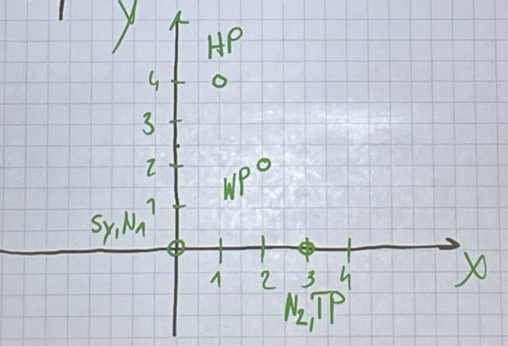
\includegraphics[scale=0.79]{Bilder/KV_1.png}
	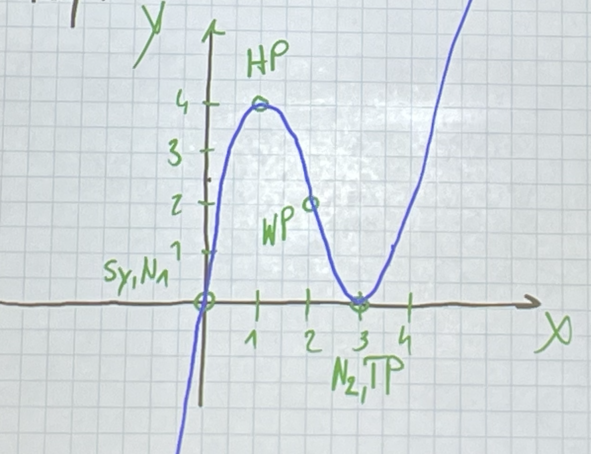
\includegraphics[scale=0.6]{Bilder/KV_2.png}
	\caption{Man sollte zuerst die bekannten Punkte einzeichnen und anhand dieser den Graphen vervollständigen}
	\end{figure}
	b) $f(x)=\frac{1}{9}x^3-\frac{1}{3}x^2-\frac{8}{3}x+\frac{26}{9}$ (Nullstelle: x=1) In diesem Beispiel wird nicht mehr die gesamte Kurvendiskussion durchgeführt, sondern nur Punkt 5 abgehandelt, da es hier vonnöten ist eine Polynomdivision durchzuführen. \\
	5. \textbf{Schnittpunkt mit x-Achse - f(x)=0} \\
	Da eine Nullstelle durch die Angabe bereits bekannt ist, kann man direkt durch (x-1) dividieren (Da 1 eine Nullstelle ist und somit $x - 1\ 0$ ergibt.)
	$f(x)=\frac{1}{9}x^3-\frac{1}{3}x^2-\frac{3}{8}x+\frac{26}{9}\to $ Da es einen Wert ohne x gibt, kann man nichts herausheben. \\
	($\frac{1}{9}x^3-\frac{1}{3}x^2-\frac{8}{3}x+\frac{26}{9}):(x-1)=\nicefrac{1}{9}x^2 -\nicefrac{2}{9}x-\nicefrac{26}{9}$\\
	$-(\nicefrac{1}{9}x^3-\nicefrac{1}{9}x2)$ \\
	$--- -\nicefrac{2}{9}x^2-\nicefrac{8}{3}x$ \\
	$-(-\nicefrac{2}{9}x^2+\nicefrac{2}{9}x)$ \\
	$--- -\nicefrac{26}{9}x+\nicefrac{26}{9}$ \\
  $-(-\nicefrac{26}{9}x+\nicefrac{26}{9})$ \\
	$--- ---$ \\
	Dieses Ergebnis führt nun zu einer "Faktorisierten Funktionsvorschrift": \\
	$f(x)=(x-1)*(\nicefrac{1}{9}x^2-\nicefrac{2}{9}x-\nicefrac{26}{9})$ \verb|Aus diesen kann man nun erneut die Nullstellen bestimmen.| \\
	Laut Angabe ist 1 eine Nullstelle, da (x-1) dem Term vorsteht. Den Rest muss man mittels großer Formel auflösen: \\
	$x_{2,3}=\frac{\nicefrac{2}{9}\pm\sqrt{\nicefrac{4}{81}+\nicefrac{104}{81}}}{\nicefrac{2}{9}}\to\ x_2=6,196, x_3=-4,196$ \\
	$N_1(-4,196|0), N_2(1|0), N_3(6,196|0)$
	\subsection{Partielle Ableitung}
	Bei einer Funktion mit mehreren Variablen, hat man nicht mehr eine zweidimensionale, sondern eine dreidimensionale Fläche. Solche Funktionen können wie: $f(x,y)=2x+y$ aussehen. Diese kann man auch ableiten, wobei man jedoch nur eine der beiden Variablen ableitet. (Man kann jedoch entweder nach x oder y ableiten.) \\
	Die Variable die nicht abgeleitet wird, verhält sich dabei wie eine Konstante. \\
	Wenn man also diese Funktion ableiten würde, erhält man $x:f_x$
	\subsubsection{Partielle Ableitungen höherer Ordnung}
	Man kann bei einer partiellen Ableitung auch mehrfach ableiten. 
	Erste Ordnung: $f(x,y)=x^2+xy+2x^2\to\ f_x(x,y)=2x+y, f_y(x,y)=x+4y$ \\
	Zweite Ordnung: $f_{xx}(x,y)=2$, $f_{yx}(x,y)=1$,\ $f_{xy}(x,y)=1, f_{yy}(x,y)=4$ \\
	Hierbei ist zur beachten, dass die Reihenfolgen der einzelnen partiellen Ableitungen austauschbar sind. Das ist auch ersichtlich, da die Ableitungen yx und xy jeweils 1 ergeben. \\
	Beispiel: \\
	11) Berechnen sie sämtliche partielle Ableitungen erster und zweiter Ordnung. \\
	b. \textbf{$f(x,y)=x^2y^3+2x+4y$} \\
	$f_x(x,y)=2xy^3+2$ \\
	$f_y(x,y)=3x^2y^2+4$ \\
	$f_{xx}(x,y)=2y^3$ \\
	$f_{xy}(x,y)=6xy^2$ \\
	$f_{yx}(x,y)=6xy^2$ \\
	$f_{yy}(x,y)=6x^2y$ \\
	\section{Integralrechnung}
	Mit der Integralrechnung kann man den Flächeinhalt einer nicht gerade verlaufenden Linie berechnen. Dabei funktioniert der Vorgang auf die gleiche Weise wie bei der Ableitung. Während man bei der Ableitung jedoch die Krümmung berechnen will und deshalb unendlich viele Tangenten bildet, will man bei dem Integral die Summe bilden und erzeugt deshalb unendlich viele Flächen unter der Linie um die Krümmung abzubilden.
	\subsection{Bestimmtes Integral}
	Bei dem bestimmten Integral wird zwischen zwei bestimmten Intervallen integriert: $\int_{a}^{b}$. Später gibt es auch unbestimmte Integrale ohne Grenzen. \\
	\subsubsection{Stammfunktion}
	Die Stammfunktion ist die Ursprungsfunktion einer Integralfunktion: $F'\to\ f$. Somit ist es erneut das Gegenstück zur Differenzierung. Während man bei der Differenzierung von einer Funktion f auf eine abgeleitete Funktion f' kommt, ist es bei dem Integral umgekehrt und man will von der Stammfunktion F' auf die Integralfunktion f kommen. \\
	Da bei dem ableiten jedoch Konstanten verloren gehen, muss man bei dem Integrieren diesen berücksichtigen. Da man jedoch nicht weiß, was diese Konstante war, schreibt man im allgemeinen den Wert c. \\
	$f(x)=x^2\to\ f'(x)=2x$ \\
	$f(x)=x^2+4\to\ f'(x)=2x$ \verb|Da beide dieser Funktionen zur selben Ableitung führen, kann man die Konstante nicht finden.|\\
	$F(x)=x^2+c\to\ f(x)=2x$ \\
	$f(x)=\frac{1}{x^3}=x^{-3}\to\ F(x)=\frac{1}{-2}x^{-2}=-\frac{1}{2x^2}+c$ \\
	\subsubsection{Hauptsatz}
	Der Hauptsatz der Integralrechnung besagt, dass bei einer stetigen Funktion der Integral gleich der Differenz des Wertes der Stammfunktion an der oberen \textbf{minus} des Werts der Stammfunktion an der unteren Integrationsgrenze ist: $\int_{a}^{b}f=F(b)-(F(a))$. \\
	Die Schreibweise für diese Differenz ist: $\int_{a}^{b}f(x)dx=[F(x)]^b_a=F(x)|^b_a=F(b)-F(a)$. \\
	Also ist das Integral die Stammfunktion zwischen den Werten a und b \\
	Beispiel: \\
	Flächeninhalt von $f(x)=x^3$ wird gesucht, a=1, b=2 \\
	$\int_{1}^{2}x^3dx=[\frac{1}{4}x^4]^2_1=\frac{1}{4}x^4|^2_1=(\frac{1}{4}2^4)-(\frac{1}{4}1^4)=4-\frac{1}{4}=3\frac{3}{4}$ \\
	Wenn Integrationsgrenzen gegeben sind, zieht man ja beide Stammfunktionen voneinander ab, wodurch bei beiden die Konstante c gegeben ist. Dadurch fällt das c am Ende weg, wodurch man es generell weglassen kann. Das ist jedoch nur bei bestimmten Integralen der Fall.
	\subsubsection{Rechenregeln}
	Bei Integralen, in welchen b größer als a ist, gilt:
	\begin{itemize}
		\item{Wenn man von a bis a integriert ist das Ergebnis stets 0: $\int_{a}^{a}f(x)dx=0$}
		\item{Wenn man von b bis a integriert, erhält man das selbe Ergebnis als bei a bis b, aber mit negativem Vorzeichen:$\int_{b}^{a}f(x)dx=-\int_{a}^{b}f(x)dx$}
	\end{itemize}
	Faktorregel:
	\begin{flalign*}
	\int_{a}^{b}c*f=c*\int_{a}^{b}f && 
	\end{flalign*}
	Summenregel:
	\begin{flalign*}
	\int_{a}^{b}(f+g)=\int_{a}^{b}f+\int_{a}^{b}g &&
	\end{flalign*}
	Intervalladditivität:
	\begin{flalign*}
	\int_{a}^{b}f=\int_{a}^{c}f+\int_{c}^{b}f\ bei\ (a < c < b) &&
	\end{flalign*}
	\subsection{Unbestimmtes Integral}
	Bei unbestimmten Integralen ist man nicht auf ein einzelnen Intervall beschränkt, wodurch man auch immer das c als Konstante hinzufügen muss.
	\subsubsection{Rechenregeln}
	$\int 0dx=c$ \verb|Das Integral von 0 ist stets die Konstante c| \\
	$\int 1dx=x+c$ \verb|Das Integral einer Konstanten ist x plus die Konstante c| \\
	$\int x^ndx=\frac{c^{n+1}}{n+1}+c$ für alle $n\ne -1$ \\
	$\int e^xdx=e^x+c$ \verb|Das Integral von der eulerschen Zahl ist die eulersche Zahl plus die Konstante c| \\
	$\int e^{kx}dx=\frac{e^{kx}}{k}+c$ \verb|Enthält die eulersche Zahl eine konstante wird diese als Divisor hinzugefügt.| \\
	$\int a^xdx=\frac{a^x}{\ln a}+c$ \verb|Das Integral eines Exponenten ist der Exponent durch den ln der Basis| \\
	$\int \frac{1}{x}dx=\ln x+c$ \verb|Das Integral von 1/x ist der ln von x| \\
	$\int \cos(x)dx = \sin(x)+c$ \verb|Das Integral des Cosinus ist der Sinus| \\
	$\int \sin(x)dx = -\cos(x)+c$ \verb|Das Integral des Sinus ist der negative Cosinus| \\    
	Beispiele: \\
	$f(x)=x^3$ \\
	$\int x^3dx=\frac{1}{4}x^4+c\to\ F(x)=\frac{1}{4}x^4+c$ \verb|Der Exponent wird um 1 erhöht und durch 4 dividiert.| \\
	\subsection{Integrationsmethoden}
	Wenn keine direkte Integration möglich ist, muss man eine der Integrationsmethoden anwendenn
	\subsubsection{Partielle Integration (Produktintegration)}
	Diese Regel wird über die Produktregel der Differentialrechnung hergeleitet: $(f*g)'=f'*g+f*g'$ \\
	Wenn also f und g differenzierbar und f' und g' stetig sind, kann man es aufsplitten: $f*g=\int f'*g+\int f*g'$ \\
	Eine dieser Integrale kann man nun auf die andere Seite bringen: $\int f*g'=f*g-\int f'*g$ \\
	Für diese Operation sollte man eine Funktion g nehmen, welche sich relativ leicht integrieren lässt. Welcher Faktor als g und f' gewählt wird ist dabei egal. So weiß man f und g, muss g integrieren und f ableiten und kann so ein weiteres Integral berechnen. Da man somit aber erneut auf ein Integral kommt, nennt man es nur partielle Integration. Es kann sein, dass man auch erneut partiell Integrieren muss. \\
	Beispiel 1: \\
	$\int x*e^xdx$ \verb|Keine bekannte Integrationsregel, aber zwei Faktoren welche multipliziert werden.| \\
	Da $e^x$ sehr einfach zu integrieren ist (Da es wieder $e^x$ ist), wählt man es als g. f lässt sich auch sehr leicht ableiten, da die Ableitung von x, 1 ist. Nun kann man mit der partiellen Integration beginnen. \\
	$\int f*g'=f*g-\int f'*g \to\ \int x*e^xdx=x*e^x-\int 1*e^xdx=x*e^x-\int e^xdx=x*e^x-e^x+c=e^x(x-1)+c$  \\
	Beispiel 2: \\
	$\int \ln(x)dx$ \verb|ln(x) hat keine Integrationsregel, weshalb ein Trick angewandt werden muss.| \\
	Da ln(x) alleine keine Regel hat, kann man für die partielle Integration 1 einsetzen. \\
	$\int \ln(x)*1dx=\ln(x)*x-\int\frac{1}{x}*xdx=\ln(x)*x-\int 1dx=\ln(x)*x-x+c=x(\ln(x)-1)+c$ \\
	Beispiel: Ermitteln Sie folgende unbestimmte Integrale mittels partieller Integration. \\
	a) $\int 10x*e^{-5x}dx\to\ f(x)=10x, f'(x)=10/g'(x)=e^{-5x}, g(x)=\frac{e^{-5x}{-5}}=-\nicefrac{1}{5}e^{-5x}$ \\
	$\int 10x*e^{-5x}dx=10x*(-\nicefrac{1}{5}e^{-5x})-\int 10*(-\nicefrac{1}{5}e^{-5x})dx$ \\
	$=-\frac{10}{5}x*e^{-5x}+\frac{10}{5}+\int e^{-5x}dx=-2xe^{-5x}+2*\frac{e^{-5x}}{-5}+c=-2xe^{-5x}-\frac{2}{5}e^{-5x}+c=-2e^{-5x}(x+\nicefrac{1}{5}+c)$
	\subsubsection{Substitutionsmethode}
	Gleich wie die partielle Integration über die Produktregel hergeleitet wird, kann die Substitutionsmethode über die Kettenregel hergeleitet werden: $(f(g))'=f'(g)*g'$ \\
	Wenn g in[a,b] und f in [g(a),g(b)] stetif und differenzierbar und g' in [a,b] stetig sind: $\int_{a}^{b}f(g(x))*g'(x)dx=\int_{g(a)}^{g(b)}f(t)dt$. Hierbei wird der innere Teil des Integral durch t substitutioniert. Wichtig für die Durchführung der Methode ist das erkennen des inneren Teils, welcher substitutioniert werden soll. \\
	Beispiel: \\
	$\int e^{x^3}*3x^2dx$ \verb|Da der innere Faktor 3x^2 die Ableitung von x^3 ist, bietet es sich an die Kettenregel zu verwenden.| \\
	$t=x^3 \verb|Inneren Faktor bestimmen|\\
	t'=3x^2 \verb|Diesen ableiten|\\
	t'=\frac{dt}{dx} \verb|Die Ableitung mit t' gleichsetzen|\\
	3x^2=\frac{dt}{dx} \verb|und einsetzen|\\
	dx=\frac{dt}{3x^2}$ \verb|Umformen sodass es auf dx aufgelöst wird und in das Integral einsetzen.|\\
	$\int e^{x^3}*3x^2dx=\int e^t*3x^2dx=\int e^t*3x^2\frac{dt}{3x2}=\int e^tdt=e^t+c$ \verb|Nun müssen die ursprünglichen Werte erneut eingesetzt werden.| \\
	Rücksubstitution: $e^t+c=e^{x^3}+c$
	Beispiel - Ermitteln Sie die folgenden Integrale mittel Substitution: \\
	a) $\int \frac{1}{5x-7}dx\to\ t=5x-7\to\ t'=5=\frac{dt}{dx}\rightarrow dx=\frac{dt}{5}$ \\
	$\int \frac{1}{5x-7}dx=\int \frac{1}{t}*\frac{dt}{5}=\frac{1}{5}*\int \frac{1}{t}dt=\nicefrac{1}{5}*\ln(t)+c$\\
	Rücksubstitution: $\nicefrac{1}{5}*\ln(t)+c=\nicefrac{1}{5}*\ln(5x-7)+c$ \\
	b)$\int_{0}^{1}\frac{x}{\sqrt{2+x^2}}dx=\int_{0}^{1}\frac{1}{\sqrt{2+x^2}}*x+dx$ \\
	$t=2+x^2, t'=2x=\frac{dt}{dx}\rightarrow dx=\frac{dt}{2x}$ \\
	Da dieses Integral bestimmt ist und bei der Substitutionsregel sich die Integrationsgrenzen verschieben, gibt es einen Trick um dies zu umgehen. Dabei wandelt man das bestimmte Integral vorübergehend in ein unbestimmtes um und setzt danach ein. \\
	$\int \frac{x}{\sqrt{2+x^2}}dx=\int \frac{\cancel{x}}{\sqrt{t}}*\frac{dt}{2\cancel{x}}=\frac{1}{2}*\int\frac{1}{\sqrt{t}}dt=\frac{1}{2}*\int \frac{1}{t^{\nicefrac{1}{2}}}dt=\frac{1}{2}+\int t^{-\nicefrac{1}{2}}dt=\cancel{\frac{1}{2}}*\frac{t^{\nicefrac{1}{2}}}{\cancel{\frac{1}{2}}}+c=t^{\nicefrac{1}{2}}+c=\sqrt{t}+c=\sqrt{2+x^2}+c=F(x)$ \\
	Nun kann man wieder in das bestimmte Integral einsetzen. \\
	$\int_{0}^{1}\frac{x}{\sqrt{2+x^2}}dx=[F(x)]^1_0=[\sqrt{2+x^2}]^1_0=\sqrt{2+1^2}-\sqrt{2+0^2}\approx0,32$
	\subsubsection{Partialbruchzerlegung}
	Bei einer Partialbruchzerlegung sind zwei Funktionen, welche dividiert werden: $f(x)=\frac{p(x)}{q(x)}$. Dabei ist die Vorraussetzung, dass sowohl p(x) als auch q(x) Polynomfunktionen sind. q(x) muss ebenfalls einen kleineren Grad als p(x) haben, also muss der Polynom im Zähler einen kleineren Grad haben als der Polynom im Nenner. \\
	Im ersten Schritt soll man so die Funktion zu Teilbrüchen umzuformen: $f(x)=\frac{p(x)}{q(x)}=\frac{p(x)}{(x-x_1)(x-x_2)...(x-x_n)}=\frac{A_1}{x-x_1}+\frac{A_2}{x-x_2}+...+\frac{A_n}{x-x_n}$ \\
	Davor muss man jedoch einige Fälle bestimmen: \\
	Im ersten Fall, wenn q(x) nur einfacher Nullstellen hat, also keine doppelten Nullstellen, kann man $A_1$ bis $A_n$ durch Koeffizientenvergleich ermitteln. $\int \frac{A_i}{x-x_i}dx=A_i*\ln(|x-x_i|)+c$ \\
	Im zweiten Fall, falls es mehrfache Nullstellen hat, muss man für jede der Nullstellen diese separat addieren, dieser Fall findet jedoch in dieser Vorlesung nicht statt. \\
	Beispiel - Ermitteln Sie die folgenden unbestimmten Integrale mittels Partialbruchzerlegung: \\
	a) $\int \frac{2x-4}{x^2-2x-8}dx\to\ f(x)=\frac{p(x)}{q(x)}=\frac{2x-4}{x^2-2x-8}$ \\
	Zuerst muss man die Nullstellen von q(x) ermitteln: $x^2-2x-8=0\to\ x_{1,2}=\frac{2\pm\sqrt{4+32}}{2}=\frac{2\pm6}{2}\to\ x_1=4, x_2=-2$\\
	Diese kann man danach in Linearfaktoren zerlegen: f(x)=$\frac{2x-4}{(x-4)*(x+2)}$ \\
	Nun muss man die A Werte mittels Koeffizientenvergleich ermitteln: $f(x)=\frac{A_1}{x-x_1}+\frac{A_2}{x-x_2}=\frac{A_1}{x-4}+\frac{A_2}{x+2}$. \\
	$=\frac{A_1*(x+2)+A_2*(x-4)}{(x-4)(x+2)}=\frac{A_1*x+2*A_1+A_2*x-4*A_2}{(x-4)(x+2)}$ Da die Ursprungsfunktion 2x-4 war, sind beide Teile in dem Bruch vorhanden. \\
	$=\frac{(A_1+A_2)*x+2A_1-4A_2}{(x-4)(x+2)}$. Umgeformt weiß man nun, dass $A_1+A_2$ 2 sein muss und $2A_1-4*A_2$ -4 sein muss. So kann man nun zwei Gleichungssysteme erstellen: \verb|I|$a_1+A_2=2$, \verb|II|$2A_1-4*A_2=-4$. Diese kann man nun separat auflösen. \\
	$f(x)=\frac{A_1}{x-4}+\frac{A_2}{x+2}=\frac{\frac{2}{3}}{x-4}+\frac{\frac{4}{3}}{x+2}$ \verb|Nun weiß man A1 und A2 und kann es berechnen.| \\
	Die Formel ist: $\int \frac{A_1}{x-x_i}dx=A_i*\ln(|x-x_i|)+c\to\ \int f(x)dx=\frac{3}{2}*\ln(|x-4|)+\frac{4}{3}*\ln(|x+2|)+c$
	\subsection{Flächenberechnung bei negativen Flächen}
	Wir haben bereits kennengelernt wie man die Fläche in einem Intervall berechnet. Diese Methode funktioniert jedoch nur, wenn der Intervall positiv ist, da sonst eine negative Fläche entstehen würde. Wenn man sich erneut die Funktion $f(x)=x^3$ ansieht, aber diesmal im Intervall $a=-1, b=1$ bestimmen will, kann man nicht die normale Formel verwenden:$\int_{-1}^{1}x^3dx=[\frac{1}{4}x^4]^1_{-1}=\frac{1}{4}x^4|^1_{-1}=(\frac{1}{4}1^4)-(\frac{1}{4}(-1)^4)=\frac{1}{4}-\frac{1}{4}=0$. Jetzt ist die berechnete Fläche 0, was jedoch nicht viel Sinn macht. Wenn man eine Fläche berechnet, muss die FLäche zwangsmäßig größer als 0 sein. Das Problem ist hierbei, dass die beiden Flächeninhalte im negativen und positiven Bereich gleich sind, wodurch sie sich aufheben und 0 entsteht. Diesen Wert nennt man allgemein den Integralwert, welcher gleich der Fläche sein kann (Wenn der Intervall positiv ist) aber nicht muss. \\
	Um dieses Problem zu umgehen muss man mehrere Intervalle berechnen: \\
	$A_1=\int_{a}^{c}f(x)dx=|\int_{a}^{c}f(x)dx|$ \\
	$A_2=-\int_{c}^{d}f(x)dx=|\int_{c}^{d}f(x)dx|$ \\
	$A_3=\int_{d}^{b}f(x)dx=|\int_{d}^{b}f(x)dx|$ \\
	Der allgemeine Vorgang für beliebige Funktionen ist:
	\begin{enumerate}
		\item{Bestimmen der Nullstellen an der Funktion}
		\item{Überprüfen, welche Nullstellen im relevanten Intervall liegen}
		\item{Optional: Überprüfen ob Vorzeichenwechsel stattfindet}
		\item{Jeden Abschnitt separat integrieren}
	\end{enumerate}
	Beispiel: Berechnen sie den Gesamtinhalt aller Flächen zwischen der x Achse und dem Graph der Funktion f im Intervall [a,b]: \\
	a) $f(x)=x^2-1$ mit a=-1 und b=2 \\
	Zuerst muss man die Nullstellen berechnen: $f(x)=0\to\ x^2-1=0\to\ x=\pm\sqrt{1}\to\ x_1=1, x_2=-1$ \\
	T[TODO] Beispiel \\
	Beispiel: Berechnen Sie den Gesamtinhalt der Flächen, die vom Graphen der Funktion f und der x-Achse eingeschlossen werden: \\
	a) $f(x)=x^3-3x^2+2x$ \verb|Nullstellen berechnen| \\
	$f(x)=0\to\ x^3-3x^2+2x=0\to\ x(x^2-3x+2)=0\to\ x^2-3x+2=0 \rightarrow x_{2,3}=\frac{3\pm\sqrt{9-8}}{2}=\frac{3\pm1}{2}\rightarrow x_1=0, x_2=2, x_3=1$. \\
	Da wir nun wissen, dass jeweils zwei Flächen eingeschlossen sind, müssen wir die Flächen dieser berechnen. \\
	$A=|\int_{0}^{1}(x^3-3x^2+2x)dx|+|\int_{1}^{2}(x^3-3x+2x)dx|=|[\frac{x^4}{4}-\cancel{3}\frac{x^3}{\cancel{3}}+\cancel{2}\frac{x^2}{\cancel{2}}]^1_0|+|[\frac{x^4}{4}-x^3+x^2]^2_1=|(\frac{1}{4}-1+1)-(0-0+0)|+|(\frac{2^4}{4}-2^3+2^2)-(\frac{1}{4}-\cancel{1}+\cancel{1})=|\frac{1}{4}|+|4-8+4-\frac{1}{4}|=\frac{2}{4}=\frac{1}{2}$FE
	\subsection{Flächen zwischen zwei Funktionen}
	Man kann auch die Fläche zwischen zwei Flächen integrieren indem man die Fläche einer Funktion von der anderen abzieht: $A=\int_{a}^{b}{f(x)-g(x)]dx}$ \\
	Beispiel - Berechnen Sie den Gesamtinhalt der Flächen, die von den Graphen der Funktionen f und g eingeschlossen werden: \\
	a) $f(x)=x^2, g(x)=2-x^2$ \verb|Zuerst muss man die Schnittstellen bestimmen| \\
	$f(x)=g(x)\to\ x^2=2-x^2\to\ 2x^2=2\to\ x=\pm\sqrt{1}\rightarrow x_1=-1, x_2=1$ \\
	$A=\int_{-1}^{1}[g(x)-f(x)]dx=\int_{-1}^{1}[2-x^2-(x^2)]dx=\int_{-1}^{1}[2-2x^2]dx=[2x-2*\frac{x^3}{3}]^1_-1=[2-\nicefrac{2}{3}]-[-2+\nicefrac{2}{3}]=2-\nicefrac{2}{3}+2-\nicefrac{2}{3}=4-\nicefrac{4}{3}=\nicefrac{12}{3}-\nicefrac{4}{3}=\nicefrac{8}{3}$FE \\
	Jedoch macht es auch keinen Unterschied, wenn man die größere von der kleineren abzieht, da man dann zwar einen negativen Wert erhält, aber es der gleiche Wert ist, nur mit einem anderen Vorzeichen.
	$A=\int_{-1}^{1}[f(x)-g(x)]dx=\int_{-1}^{1}[x^2-(2-x^2)]dx=\int_{-1}^{1}[2x^2-2]dx=[2\frac{x^3}{3}-2x]^1_1=[\frac{2}{3}-2]-[-\frac{2}{3}+2]=\frac{2}{3}-2+\frac{2}{3}-2=\frac{4}{3}-4=\frac{4}{3}-\frac{12}{3}=-\frac{8}{3}$
	\subsection{Rotationsvolumen}
	Ein Rotationskörper ist ein Körper welcher entsteht, indem eine Kurve um eine Achse rotiert wird. \\
	Bei der Rotation um die x Achse kann das Volumen eines solchen Körpers mit $V=\pi \int_{a}^{b}(f(x))^2dx$ berechnet werden. Diese Formel rührt daher, dass der Körper aus unendlich vielen Kreisen besteht, welche danach aufsummiert werden. \\
	Es kann jedoch auch um die y Achse rotiert werden, indem man die Umkehrfunktion berechnet. $V=\pi \int_{f(a)}^{f(b)}f^{-1}(x))^2dx$ \\
	Beispiel 7 - Berechnen Sie das Volumen das entsteht, wenn man den Graphen der Funktion f im Intervall [a,b] um die x-Achse rotieren lässt: \\
	a) $f(x)=x,\ a=0,\ b=2$ - Rotationsvolumen um die x-Achse - $V=\pi*\int_{a}^{b}(f(x))^2dx$ \\
	$=\pi \int_{0}^{2}x^2dx=\pi*[\frac{x^3}{3}]^2_0$ \\
	$=\pi*[\frac{2^3}{3}-\frac{0^3}{3}]=\pi*\frac{8}{3}=\frac{8}{3}\pi$FE \\
	Beispiel 8 - Leiten Sie die Volumensformel eines Kreiskegels $V=\frac{1}{3}*\pi*r^2*h$ mittels Integralrechnung her. \\
	In einem Kreiskegel ist der Funktionswert im gesuchten Bereich die Seitenlänge des Kegels. Der Radius des Kegels ist dabei der Wert der Funktion an der größten Stelle und die Höhe die Differenz der x Werte der Funktionsenden. Die Steigung kann somit mit $\frac{r}{h}$ berechnet werden, da ein Steigungsdreieck stets mit $\frac{\Delta y}{\Delta x} $berechnet werden kann. \\
	Da wir wissen, dass ein Kegel eine Gerade als Seitenlänge hat, handelt es sich um eine lineare Funktion $f(x)=kx+d$. Die Funktion in diesem Fall lautet dann $f(x)=\frac{r}{h}x$ wobei von 0 bis h integriert wird: $a=0,\ b=h$. \\
	Jetzt kann man in die Volumensformel einsetzen: $V=\pi*\int_{a}^{b}(f(x))^2dx=\pi*\int_{0}^{h}(\frac{r}{h}x)^2dx$ \\
	$=\pi \int_{0}^{h}\frac{r^2}{h^2}x^2dx=\pi*\frac{r^2}{h^2}*\int_{0}^{h}x^2dx$ \\
	$=\pi*\frac{r^2}{h^2}*[\frac{x^3}{3}]_0^h=\pi \frac{r^2}{\cancel{h^2}}*[\frac{h^{\cancel{3}}}{3}]$ \\
	$=\frac{1}{3}*\pi*r^2*h$ \\
	Beispiel 9 - Berechnen Sie das Rotationsvolumen um die y-Achse: \\
	a) $f(x)\nicefrac{1}{2}x^2,\ a=1,\ b=3$ \\
	Um das Volumen um die y-Achse zu berechnen muss man die Umkehrfunktion der Funktion berechnen. Dafür muss die Funktion jedoch bijektiv sein, was diese Funktion nicht ist. Da wir jedoch nur an dem Bereich 1 bis 3 interessiert sind, muss nur dieser Teil bijektiv sein, was er auch ist. \\
	$f^-1(x):y=\nicefrac{1}{2}x^2\to\ x^2=2y\to\ x=\sqrt{2y}\to\ y=\sqrt{2x}\to\ f^-1{x)=\sqrt{2x}}$ \\
	Um das y-Volumen zu berechnen muss man nun noch die Integrationsgrenzen zu f(a) und f(b) verschieben: $V=\pi \int_{f(a)}^{f(b)}(f^-1(x))^2dx$. Diese Grenzen sind: $f(a)=f(1)=\nicefrac{1}{2}*1^2=\nicefrac{1}{2}$ und $f(b)=f(3)=\nicefrac{1}{2}*3^2=\nicefrac{9}{2}$ \\
	Also ist die Funktion: $\pi \int_{\nicefrac{1}{2}}^{\nicefrac{9}{2}}(\sqrt{2x})^2dx$ \\
	$=\pi \int_{\nicefrac{1}{2}}^{\nicefrac{9}{2}}2xdx=\pi*[\cancel{2}*\frac{x^2}{\cancel{2}}]^{\nicefrac{9}{2}}_{\nicefrac{1}{2}}$\\
	$=\pi*[(\nicefrac{9}{2})^2-(\nicefrac{1}{2})^2]=\pi[\nicefrac{81}{4}-\nicefrac{1}{4}]=\pi*\frac{80}{4}=20\pi$VE
	\subsection{Bogenlänge}
	Man kann ein Integral auch zur Berechnung von Parabel- und Brückenbögen verwenden. Die Bogenlänge ist dabei die Länge eines Bogens in einem bestimmten Interval [a, b]. Die Bogenlänge wird berechnet mit $L=\int_{a}^{b}\sqrt{1+(f'(x))^2}dx$. Also ist die Bogenlänge die Integration der Ableitung des Bogens. \\
	Beispiel 10 - Berechnen Sie die Bogenlänge des Graphen der Funktion f im Intervall [a,b]: \\
	a) $f(x)=\frac{1}{2}(e^x+e^{-x}),\ a=0, b=2$ \verb|-> Zuerst muss abgeleitet werden.| \\
	$f(x)=\nicefrac{1}{2}e^x+\nicefrac{1}{2}e^{-x}\to\ f'(x)=\nicefrac{1}{2}e^x+\nicefrac{1}{2}e^{-x}+(-1)$ \\
	$=f'(x)=\nicefrac{1}{2}e^x-\nicefrac{1}{2}e^{-x}$ \verb|Jetzt muss man nur mehr in die Formel einsetzen| \\
	$L=\int_{a}^{b}\sqrt{a+(f'(x))^2}dx\to\ \int_{0}^{2}\sqrt{1+(\nicefrac{1}{2}(e^x-e^{-x})^2}dx$ \\
	$=\int_{0}^{2}\sqrt{1+(\nicefrac{1}{4}(e^{2x}-\cancel{2}e^x*\cancel{e^{-x}}+e^{-2x}))}dx$ \\
	$=\int_{0}^{2}\sqrt{1+(\nicefrac{1}{4}e^{2x}-\nicefrac{1}{2}+\nicefrac{1}{4}e^{-2x})}dx=\int_{0}^{2}\sqrt{\nicefrac{1}{2}+\nicefrac{1}{4}e^{2x}+\nicefrac{1}{4}e^{-2x}}dx$ \\
	$=\int_{0}^{2}\sqrt{\nicefrac{1}{4}(2+e^{2x}+e^{-2x})}dx$ \verb|-> Kann in eine binomische Formel umgewandelt werden| \\
	$=\int_{0}^{2}\sqrt{\nicefrac{1}{4}(e^x+^{-x})^2}=\int_{0}^{2}\nicefrac{1}{2}(e^x+^{-x})dx$ \verb|1/2 kann als Konstante isoliert werden| \\
	$=\nicefrac{1}{2}\int_{0}^{2}(e^x+e^{-x})dx=\nicefrac{1}{2}*[e^x+\frac{e^{-x}}{-1}]_0^2$ \\
	$=\nicefrac{1}{2}*[e^2-e^{-2}-\cancel{(e^0-e^{-0})}]=\nicefrac{1}{2}(e^2-e^{-2})\approx 3,63$LE (Längeneinheiten)

	










\end{document}